\documentclass[]{mgr}

\usepackage{polski}

\usepackage[utf8]{inputenc}
\usepackage[T1]{fontenc}

\usepackage{graphicx}
\usepackage{caption}
\usepackage{subcaption}

\usepackage{wrapfig}
\usepackage{psfrag}

\usepackage{amsmath}
\usepackage{amsfonts}
\usepackage{amssymb}

\usepackage{listings}
\usepackage{url}

\title{System ekspertowy dopasowujący wskazania systemu DXCluster do potrzeb użytkowników}
\engtitle{Expert system for matching DXCluster system to identify the needs of users}
\author{Paweł Marcin Szwagierek}
\supervisor{dr inż. Jerzy Greblicki, I-6}
\date{2015}

\field{Informatyka (INF)}
\specialisation{Inżynieria Internetowa (INT)}

\makeatletter
\def\@makechapterhead#1{%
  \vspace*{50\p@}%
  {\parindent \z@ \raggedright \normalfont
    \ifnum \c@secnumdepth >\m@ne
      \if@mainmatter
        \Huge\bfseries \thechapter.\space%
      \fi
    \fi
    \interlinepenalty\@M
    \Huge \bfseries #1\par\nobreak
    \vskip 40\p@
  }}
\makeatother

\begin{document}
    \bibliographystyle{plabbrv}
    \maketitle

    \tableofcontents

    \chapter{Wstęp}
    TODO

    \chapter{Problematyka amatorskich systemów radiowych}
    \label{sec:teoretical_description}
    W pierwszym rozdziale zostaną wprowadzone podstawowe pojęcia z dziedziny krótkofalarstwa, jego możliwości, zakres działań radioamatorów.

        \section{Radioamator}
        Cała dziedzina krótkofalarstwa nie miałaby sensu gdyby nie amatorzy zafascynowani radiokomunikacją, pasjonaci łączności lokalnych oraz łączności dalekiego zasięgu a także naukowcy i specjaliści ciągle udoskonalający istniejące projekty. W ogromnej większości radioamatorzy to osoby zajmujące się radiotechniką niezawodowo. Istnieją radioamatorzy bierni, poprzestający na studiowaniu samego tematu krótkofalarstwa, rzadko wkraczający w~dziedzinę praktyki radioamatorskiej. Amatorzy czynni na podstawie zezwolenia odpowiednich władz budują i~uruchamiają własne, indywidualnie lub zbiorowo (działając w~różnego rodzaju klubach), krótkofalowe i~ultrakrótkofalowe stacje nadawcze małej mocy.

        Duża część pracy radioamatora to próby, eksperymenty, budowanie swoich projektów a następnie wymiana doświadczeń z innymi. Zwykle są to wnioski na podstawie krótkich obserwacji, lecz niejednokrotnie są to duże i konkretne artykuły prezentowane w czasopismach branżowych. Wymieniane są spostrzeżenia dotyczące techniki radioamatorskiej, rozprzestrzeniania się fal elektromagnetycznych w~poszczególnych zakresach itp. Często w ten sposób społeczność radioamatorów przyczynia się do rozwoju wiedzy i~techniki. 

        \section{Krótkofalarstwo}
        Terminem krótkofalarstwo określa się hobby polegające na nawiązywaniu łączności z~innymi stacjami radioamatorskimi za pomocą nadajników radiowych. W~przypadku nowoczesnych sposobów komunikacji (np. poczta elektroniczna, komunikatory Internetowe, telefonia komórkowa), nieważny jest sposób przesłania informacji z~punktu A do punku~B, a sama informacja. W wypadku krótkofalarstwa większy nacisk kładzie się na sposób przesłania informacji (sprzęt radiowy, rodzaj emisji, pasmo, anteny itd) a także w wielu przypadkach na sam fakt przeprowadzonej łączności dalekiego dasięgu. Łączność ze stacją, która jest aktywna przykładowo jednego losowego dnia w roku może być bardzo dużym wyzwaniem. Podczas samych łączności krótkofalarskich istotnymi informacjami wymienianymi przez użytkowników stacji są ich osobiste znaki wywoławcze oraz raporty o~słyszalności i~sile odebranego sygnału, a~także wykorzystanych antenach, radioodbiornikach, programach komputerowych użytych do wykorzystania modulacji cyfrowych i innych parametrach związanych z~aktualnie przeprowadzaną łącznością. Samo krótkofalarstwo jest dziedziną zainteresowań o~bogatym wachlarzu możliwości.

            \subsection{Edukacja}
            (!!! COPIED !!!) Jednym z~korzyści jakie niesie ze sobą ten temat, to ogromna ilość wiedzy z~różnych lecz poniekąd pokrewnych sobie dziedzin. Taka wiedza może zostać przekazana uczniom szkół w~czasie zajęć obejmujących zagadnienia ściśle powiązane z~krótkofalarstwem. Bogatą wiedzę można także pozyskać uczestnicząc w~spotkaniach klubów krótkofalarskich lub uczestnicząc w~zajęciach prowadzonych przez takie kluby. Przekazywane tam informacje są najbardziej usystematyzowane. Rozwiązanie takie daje także możliwości skorzystania z~klubowych radiostacji. Ostatnim ze sposobów podjęcia takiej wiedzy jest nauka samodzielna korzystając z~rozmaitej literatury tematycznej, publikacji lub artykułów sporządzonych samodzielnie przez radioamatorów z~całego świata.

            Przede wszystkim radioamator uczy się przy okazji pasji dużo z~dziedziny telekomunikacji. Poznaje rodzaje anten, które wykorzystuje się w~pracy z~różnymi pasmami a także ich budowę. Uczy się także typów modulacji oraz rodzajów emisji. W~przypadku elektroniki krótkofalarstwo daje szansę poznania zasad działania różnych urządzeń elektronicznych oraz zagadnienia przetwarzania sygnałów. Budowanie automatycznych przełączników lub sterowników rotorów antenowych wiąże się z~poznaniem zagadnień z~dziedziny automatyki. Krótkofalarstwo wprowadza także wiele wiedzy z~zakresu informatyki, gdzie radioamator może wykorzystać do transmisji informacji różne rodzaje emisji cyfrowych lub stworzyć swój własny system SDR\footnote{SDR (ang. Software Defined Radio, radio programowalne) – system komunikacji radiowej, w~którym działanie podstawowych elementów elektronicznych (takich jak mieszacze, filtry, modulatory i~demodulatory) jest realizowane za pomocą programu komputerowego.} i~korzystać ze swojego oddalonego o~znaczną odległość radia za pośrednictwem Internetu lub dać możliwość korzystania ze swoich anten i~prowadzenia nasłuchu innym radioamatorom. Na pograniczu leżą także takie dziedziny nauki jak kryptografia, w~przypadku gdy użytkownicy dwóch stacji chcą się porozumiewać zachowując poufność przesyłanych informacji. Istotną umiejętnością jest także znajomość języków obcych. Bez tego prawie niemożliwym jest prowadzenie łączności z~radioamatorami posługującymi się innymi językami. Krótkofalarstwo wprowadza także wiele umiejętności stricte powiazanych z tą dziedziną - umiejętność komunikacji za pomocą telegrafii (alfabetem Morse'a), znajomość fonetycznej reprezentacji liter w różnych językach (\mbox{A -- Alpha/Adam}, B -- Bravo/Barbara, C -- Charlie/Celina, itd.).

            Jest to jedna z~nielicznych pasji, która pozwala na wykorzystanie w globalnych łącznościach własnoręcznie stworzonego sprzętu. Społeczność krótkofalowców popiera i~wręcz dopinguje budowanie i~wykorzystanie własnych urządzeń radiowych, anten a także pozostałego oprzyrządowania niezbędnego w~pracy lub ułatwiającego pracę radioamatora - jak na przykład przełączniki antenowe, wzmacniacze, klucze telegraficzne itp) oraz programów komputerowych - do transmisji danych różnymi typami emisji, do monitorowania pracy radioamatora lub do sterowania pracą radioodbiornika za pomocą komputera. Dodatkowym atutem jest brak konieczności posiadania jakichkolwiek homologacji lub zezwoleń na korzystanie z~własnych urządzeń, co jest ogromną zaletą w przeciwieństwie do pasm CB, gdzie urządzenie musi być homologowane i mieć określone warunki pracy lub pasm PMR (w jakich pracują na przykład proste urządzenia Walkie-Talkie), gdzie urządzenie musi być o bardzo niskiej mocy, mieć na stale przyczepioną antenę i trwale zamkniętą obudowę aby uniemożliwić ingerencję ze strony użytkowników. Najwięcej osób używa jednak urządzeń fabrycznych. Jest to droższe rozwiązanie, ale dużo łatwiejsze aby od razu zacząć komunikację z innymi.

            \subsection{Amatorska Służba Radiowa}
            Radioamatorzy posiadający urządzenia nadawczo-odbiorcze są w~stanie skomunikować się ze znaczną grupą osób w~swoim otoczeniu lub dowolnym zakątkiem kraju czy świata. To daje możliwość pomocy innym ludziom w~wymianie informacji w~sytuacjach nieprzewidzianych, nagłych wypadkach, katastrofach lub klęskach żywiołowych. Krótkofalowcy są często jedynymi, którym udaje się nawiązać łączność pomiędzy odciętymi komunikacyjnie regionami. Najlepszym przykładem może tu być przypadek powodzi jaka nawiedziła województwa Dolnośląskie oraz Opolskie w 1997 roku. Z powodu braku zasilania i awarii tradycyjnych metod komunikacji większość informacji pomiędzy ludnością cywilną przekazywana była dzięki pracy krótkofalowców. Informacje o zagnionych lub znalezionych osobach, o~stanie wody lub nadchodzących nowych zagrożeniach. Krótkofalowcy pomagali również podczas powodzi w 2007 i 2010 roku.

            Wielu radioamatorów angażuje się także w~szkolenie innych ludzi w~zakresie krótkofalarstwa lub dziedzin ściśle z~nim powiązanych. To nieoceniona pomoc dla początkujących, która pozwala łatwiej zacząć przygodę z~krótkofalarstwem i wdrożyć się tematykę bez konieczności czytania wielu potężnych tomów literatury lub czasopism branżowych.

            \subsection{Hobby}
            (!!! COPIED !!!) Najwięcej ludzi skłania się do krótkofalarstwa z~powodu hobby. Posiada wiele dyscyplin jak zawody, wyprawy, prowadzenie łączności dalekiego zasięgu, eksperymentowanie z~różnymi typami emisji lub po prostu pozostawanie w~kontakcie z~przyjaciółmi korzystając z~innego środka komunikacji od popularnych w~dzisiejszych czasach telefonii komórkowej czy Internetu.

                \subsubsection{Zawody}
                    \begin{wrapfigure}{r}{0.4\textwidth}
                        \vspace{-25pt}
                        \begin{center}
                            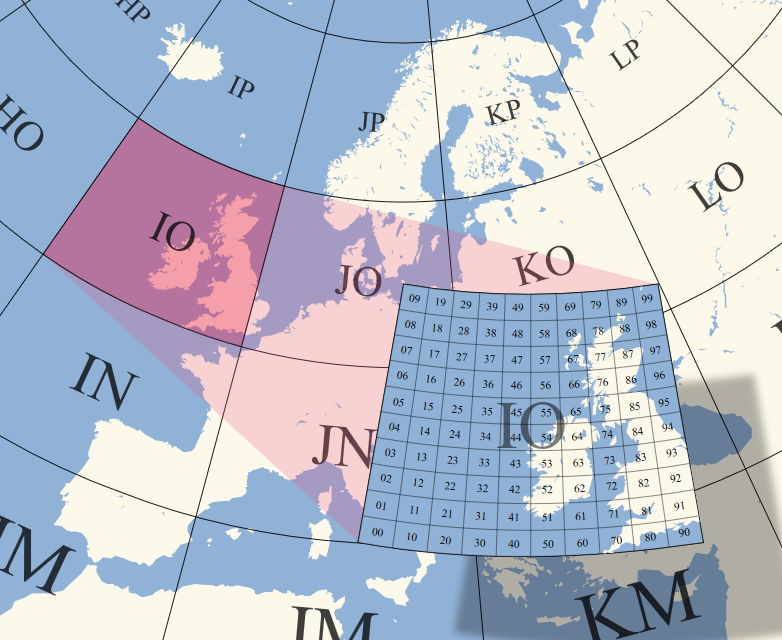
\includegraphics[scale=0.20]{gridsquare}
                        \end{center}
                        \vspace{-20pt}
                        \caption{Podział ziemi na kwadraty do określenia lokatora stacji}
                        \vspace{-10pt}
                        \label{fig:gridsquare}
                    \end{wrapfigure}
                Jedną z~dziedzin rywalizacji pomiędzy radioamatorami są zawody przeprowadzane w~ściśle określonym czasie. Polegają na nawiązaniu jak największej liczby łączności z~innymi operatorami stacji i~tym samym zdobywaniu punktów przydzielanych według zasad określonych w~regulaminie. Zaliczane są tylko bezbłędne łączności potwierdzone wymienionymi znakami wywoławczymi, raportami RST\footnote{RST (Readability, Strength, Tone) - raport oceniający Czytelność, Siłę oraz Ton aktualnie odbieranego sygnału. Składa się z trzech składowych, z których pierwsza (czytelność) oceniana jest w skali 1-5, druga (siła sygnału) w skali 1-9 i trzecia (ton - nieużywana w przypadku łączności fonicznych) w~\mbox{skali~1-9}. Najczęstszymi raportami są raporty 59 określające doskonałą czytelność odbieranych komunikatów i mocną siłę sygnału}, numerami porządkowymi łączności oraz lokatorami\footnote{Lokator (ang. Grid Square Locator) – System Lokatorów, w którym świat jest podzielony na równe kwadraty. Każdy z kwadratów jest podzielony na kolejne itd. (rys.~\ref{fig:gridsquare}). Pozycja geograficzna jest zapisywana w formacie LLCCLL - gdzie L to litera a C to cyfra. Dla przykładu lokator gmachu głównego Politechniki Wrocławskiej to JO81MC.} swojej stacji. Te dane po zakończeniu zawodów poddawane są weryfikacji przez organizatora przy pomocy programów komputerowych. Zwykle nagrodami są dyplomy dla osoby lub drużyny wygrywającej zawody.

                \subsubsection{Łączności lokalne}
                    \begin{wrapfigure}{r}{0.4\textwidth}
                        \vspace{-20pt}
                        \begin{center}
                            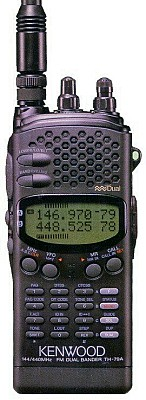
\includegraphics[scale=0.55]{ukf_handheld}
                        \end{center}
                        \vspace{-20pt}
                        \caption{Prosty nadajnik ręczny do pracy w~paśmie UKF}
                        \vspace{-20pt}
                        \label{fig:ukf_handheld}
                    \end{wrapfigure}
                Do prowadzenia łączności ze znajomymi mieszkającymi w~naszym otoczeniu wystarczy tani nadajnik przenośny, jak pokazany na rysunku~\ref{fig:ukf_handheld} lub samochodowy pracujący na pasmach UKF. Stosunkowo mała moc urządzeń pozwala na objęcie swoim zasięgiem czasami nawet całego miasta. W~przypadku gdy taki zasięg staje się niewystarczający, w~orężu radioamatorów pozostają tzw. przemienniki - urządzenia montowane na znacznych wysokościach (wysokich obiektach miejskich, wzniesieniach terenu), które odbierają sygnał i~nadają go powtórnie z~dużo większą mocą. Skutkuje to wielokrotnym zwiększeniem zasięgu prowadzonych łączności nawet do kilkuset kilometrów. Przemienniki amatorskie nie nadają cały czas, aby nie zużywały energii gdy nikt z~nich nie korzysta. W~celu skorzystania z~takiego przemiennika należy go wcześniej ,,otworzyć'' sygnałem akustycznym o~określonej częstotliwości, jednym z~tonów DTMF lub sygnałów CTCSS.

                \subsubsection{Łączności dalekiego zasięgu (DX)}
                (!!! Copied !!!) Radioamatorzy, którzy korzystają z~bardziej zaawansowanych urządzeń i~anten mogą pracować z~innymi rodzajami emisji oraz na innych pasmach (fale krótkie (KF), fale średnie). Pozwala to na realizację łączności na dużo większe odległości - opierając się na samej mocy i~charakterystyce emitowanego sygnału, wykorzystując zjawiska pogodowe, zjawisko odbicia fal lub korzystając z~amatorskich satelitów komunikacyjnych działających w~paśmie UKF. Można dzięki temu nawiązywać łączności międzykontynentalne na dystansach rzędu tysięcy kilometrów.

                    \paragraph{Fale odbite od warstw jonosfery}
                    Łączności dalekiego zasięgu na falach krótkich można zrealizować korzystając z~nadajników małej mocy i~nieskomplikowanych drutowych anten wykorzystując zjawisko odbicia fal od jonosfery. Zjawisko to występuje powszechnie i~w~zależności od pory dnia i~aktywności słonecznej umożliwia łączności na odległość od kilkuset do kilkunastu tysięcy kilometrów. Łączności z~najbardziej odległymi stacjami prowadzi się poprzez wielokrotne odbicia, niekiedy pokonujące dłuższą drogę wokół kuli ziemskiej.

                    \paragraph{Fale odbite od powierzchni księżyca}
                    Jednym z~najbardziej niezwykłych rodzajów łączności są te z~wykorzystaniem odbicia fali od powierzchni księżyca (EME). Do tego typu łączności wykorzystuje się zaawansowane systemy antenowe (jak przedstawiona na rysunku~\ref{fig:eme_antenna} oraz nadajniki o~wysokiej mocy. Przy EME wymagana jest duża precyzja oraz doświadczenie w~prowadzeniu takich łączności, przez co jest to dziedzina krótkofalarstwa która odstrasza początkujących radioamatorów. 

                    Antena powinna być skierowana dokładnie w~kierunku księżyca, który pozostaje w~ruchu względem powierzchni ziemi. W~związku z~tym aby powszechnie wykorzystywanymi są skomplikowane systemy obracania anten. W~przypadku złego ustawienia anteny najczęstszymi zakłóceniami sygnału są zniekształcenia czoła fali w~wyniku nakładania się fal odbitych. Typowymi dla tego rodzaju łączności są zjawiska odbioru własnego echa po około 2 sekundach od wysłania komunikatu oraz niewyjaśnione dotąd echo z~dużym opóźnieniem. Skutkiem tego jest otrzymanie przez nadawcę swojego komunikatu ale po czasie dochodzącym nawet do kilku minut.

                        \begin{wrapfigure}{r}{0.4\textwidth}
                            \vspace{-20pt}
                            \begin{center}
                                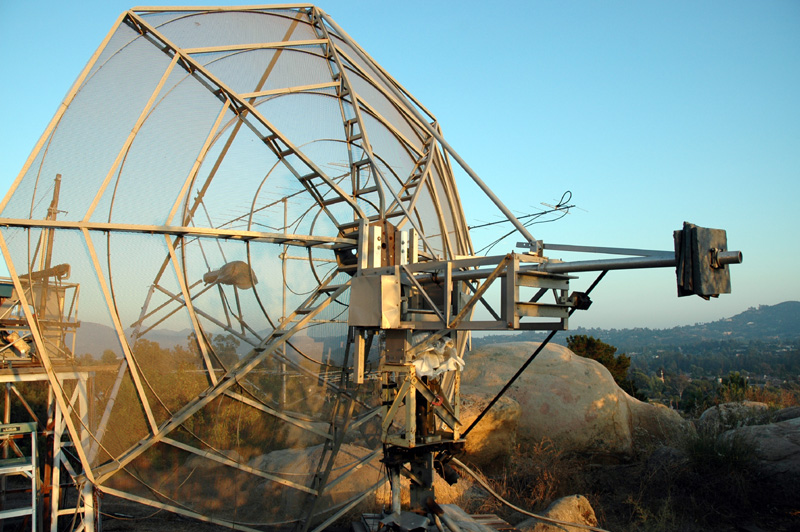
\includegraphics[width=0.4\textwidth]{eme_antenna}
                            \end{center}
                            \vspace{-20pt}
                            \caption{Antena paraboliczna wykorzystywana do łączności EME pracująca w~paśmie fal 430MHz}
                            \vspace{-20pt}
                            \label{fig:eme_antenna}
                        \end{wrapfigure}

                    Łączności wykonywane tą techniką ze względu na małą skuteczność, małą pewność transmisji oraz trudności związane z~jej wykonaniem realizują tylko radioamatorzy.

                    \paragraph{Łączności satelitarne}
                    Krótkofalowcy korzystają także ze swoich satelitów. Takich satelitów niskoorbitalnych\footnote{Satelita niskoorbitalny - satelita krążący wokół Ziemi po orbicie kołowej na wysokości 10 tys. km - 500 tys. km} jest kilkadziesiąt i~co jakiś czas wysyłane są kolejne. Fale pasma UKF pozwalają na przeprowadzenie łączności z~astronautami z~międzynarodowej stacji kosmicznej ISS a także na łączności pomiędzy radioamatorami. Korzystanie z~satelitów wymaga znajomości ich pozycji na niebie, parametrów pracy oraz ciągłego korygowania ustawienia anteny. Także sama komunikacja wygląda nieco inaczej niż w~przypadku normalnej łączności. W~przypadku satelity wiadomości nadawane są na częstotliwości zwanej ,,uplink'' i~odbierane na częstotliwości oznaczonej jako ,,downlink''. Jest to uwarunkowane zasadą pracy satelity. Odbiera ona sygnały z~jednej częstotliwości i~retransmituje te same sygnały ze zwiększoną mocą na innej częstotliwości - podobnie jak to dzieje się w~przypadku przemienników amatorskich.
                        \begin{wrapfigure}{r}{0.4\textwidth}
                            \vspace{-25pt}
                            \begin{center}
                                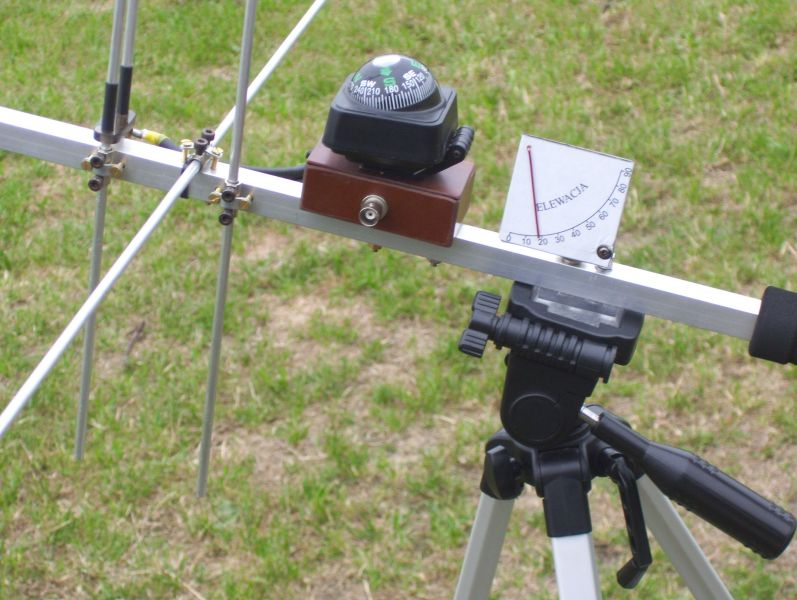
\includegraphics[width=0.4\textwidth]{example_sat_construction}
                            \end{center}
                            \vspace{-20pt}
                            \caption{Konstrukcja radioamatora SQ5RJK do ręcznego ustawiania i~korygowania pozycji anteny podczas łączności satelitarnych}
                            \vspace{-50pt}
                            \label{fig:example_sat_construction}
                        \end{wrapfigure}
                    W~związku z~tym, że pozycja anteny musi być na bieżąco korygowana, stosuje się skomplikowane systemy obracania anten lub rolę tę przejmuje sam radioamator i~pozycję anteny koryguje ręcznie korzystając z~takich konstrukcji jak pokazana na rysunku~\ref{fig:example_sat_construction}.

                    \paragraph{Inne typy łączności}
                    Sporadycznie radioamatorzy korzystają do zrealizowania łączności z~takich zjawisk jak odbicia fal radiowych od zorzy polarnej, meteorytów a nawet chmur burzowych.

                \subsubsection{Wyprawy}
                (!!! Copied !!!) W~społeczności krótkofalarskiej popularnymi są także wyprawy zwane inaczej DXpedycjami. Radioamatorzy w~pojedynkę lub w~zorganizowanej grupie wraz z~członkami klubu zdobywają górę lub niezamieszkały teren aby tam utworzyć tymczasową stację i~przeprowadzić łączności z~innymi stacjami. Taki proces często nazywany jest aktywowaniem kraju.

                \subsubsection{QSL}
                Podstawowym wymogiem do uznania każdej wykonanej łączności jest wymiana znaków wywoławczych operatorów stacji oraz wymiana raportów słyszalności i~siły sygnału. To wystarczy, żeby uznać łączność za zrealizowaną. Oficjalnym i~bardzo eleganckim potwierdzeniem łączności są karty QSL\footnote{QSL - Jeden z~symboli Kodu Q używanego w~telegrafii i~krótkofalarstwie. Domyślnym jego znaczeniem tego symbolu jest potwierdzenie łączności.}. Są wizytówkami radioamatorów oraz kartami z~dokładnym opisem zrealizowanej łączności. Dla pewnej grupy krótkofalowców stanowią one swego rodzaju trofea ze swojej służby radiowej. Wielu z~nich skupia się na ustanawianiu łączności z~jak największą ilością stacji z~odrębnych krajów. Jest to ciekawe wyzwanie z~tego powodu, że wraz ze ,,zdobywaniem'' kolejnych krajów, stopień trudności znacząco rośnie, ponieważ istnieją kraje, w~których liczba radioamatorów jest bardzo mała, region kuli ziemskiej uznany w~społeczeństwie krótkofalarskim jako kraj jest niezamieszkały lub ze względów politycznych działalność krótkofalarska nie może funkcjonować.

                Istanieją dodatkowo organizaje, które promują tego typu działaność hobbystyczną i~za szczególne osiągnięcia przyanają dyplomy. Wydawane są one na podstawie łączności potwierdzonych kartami QSL. Do najpopularniejszych dyplomów zaliczają się:
                \begin{itemize}
                    \item DX Century Club - najbardziej popularny wydawany przez ARRL\footnote{ARRL (The American Radio Relay League) - największe stowarzyszenie zrzeszające krótkofalowców i radioamatorów w USA. Jest organizacją non-profit. Dostarcza informacji technicznych, udziela pomocy entuzjastom krótkofalarstwa a także wspiera kilka programów edukacyjnych w kraju. Wydaje także dyplom DX Century Club.} dyplom świadczący o przeprowadzeniu łączności z co najmniej 100 krajami z listy DXCC.
                    \item IOTA\footnote{IOTA - ang. Islands on the Air, Wyspy w eterze} - wydawany przez Radio Society of Great Britain za łączności z wyspami i grupami wysp świata, a nie z krajami z listy DXCC. Z racji tego, że nie ma na świecie krótkofalowca, który mógłby się pochwalić potwierdzonymi łąćznościami ze wszystkimi wyspami wymienionymi w oficjalnym zestawieniu, dyplom IOTA wydawany jest za potwierdzoe łączności ze 100 wyspami oznaczonymi różnymi numerami kontrolnymi zgodnymi z przewodnikiem dyplomowym przy czym w tej liczbie musi być po jednej łączności z każdym z 7 kontynentów. Dyplom ten jest jednym z~powodów, dla których ludzie poświęcając swój wolny czas w czasie urlopu, wakacji czy emerytury organizują wyprawy na często maleńkie i niezamieszkałe wyspy aby po pierwsze daną wyspę ,,aktywować'' lub skłonić komitet do przynania wyspie odrębnego numeru. Polskimi wyspami zaliczanymi do programu IOTA są: Wolin (o~numerze EU 132) oraz Uznam (nr EU 129). Pomimo tego, że są to wyspy zamieszkałe, zostało przeprowadzonych na ich teren kilka krótkofalarskich wypraw w celu ich ,,aktywowania''.
                    \item Worked All Zones - dyplom wydawany przez czasopismo CQ Amateur Radio krótkofalowcom, którzy przeprowadzili kompletną łączność z innymi radiostacjami ze wszystkich czterdziestu stref, na które podzielony jest świat krótkofalarski.
                    \item Worked All States - dyplom sponsorowany przez ARRL, wręczany krótkofalowcom, którzy przeprowadzili kompletną i potwierdzoną łączność z innymi radiostacjami położonymi w każdym z 50 stanów USA.
                \end{itemize}

                Właśnie ta tematyka (kolekcjonowanie krajów z którymi została przeprowadzona łączność) będzie poruszona w tej pracy. Zagadnienia bardziej szczegółowo z nią powiązane zostanę opisane w kolejnym rozdziale.

    \chapter{Tematyka i problemy związane z kolekcjonowaniem krajów}
    \label{sec:collecting_entities}

    Jak w każdej dziedzinie, również w krótkofalarstwie, pojawiają się różne sfery działalności oraz zainteresowań. W każdej z nich obowiązują pewne ścisłe pojęcia, procedury a także narzędzia, z których można korzystać aby ułatwić sobie pracę. Aby skutecznie bawić się w kolekcjonowanie krajów, z którymi radioamator przeprowadził łączność, należy poznać pojęcie potwierdzenia łączności. Ważnymi są także pojęcia potrzebne do rozróżnienia obszarów w jakich dany kraj leży oraz pojęcie samego kraju, gdyż nie zawsze lista krajów pokrywa się z podziałem terytorialnym w rozumieniu państwa (na przykład USA to 15 oddzielnych krajów). Dodatkowo znacznym ułatwieniem jest dla radioamatora prowadzenie swojego logu (dziennika) wszystkich przeprowadzonych łączności. Osatatnim bardzo ważnym narzędziem przy próbach przeprowadzenia łączności dalekiego zasięgu są systemy przekazywania informacji w kręgu radioamatorów. Najpopularniejszym systemem wymiany takich informacji jest tzw. DX Cluster opisany na końcu tego rozdziału.

        \section{Metody potwierdzenia łączności}
        W przeciwieństwie do tradycyjnych metod komunikacji (poczta, telefon, Internet), w przypadku łączności radiowej nie zostaje żaden historyczny ślad potwierdzający taką łączność. W przypadku poczty mamy archiwalne listy, w przypadku telefonu operator zapisuje szczegóły połączenia (rozmówców, termin i czas), a w Internecie mamy archiwum rozmów lub zapisane e-maile.
        Aby uznać to, że łączność radiowa odbyła się poprawnie (wszystkie informacje zostały właściwie wymienione i zrozumiane przez rozmówców) oraz zapisać to jak i kiedy dana łączność się odbyła należy ją dodatkowo potwierdzić. Obecnie do potwierdzenia łączności można wykorzystać metodę tradycyjnych (papierowych) kart QSL lub metodę elektroniczną jako zapis w stworzonym do tego celu serwisie Internetowym.
        Absolutnie koniecznymi danymi do potwierdzenia łączności muszą być:
        \begin{itemize}
            \item znaki wywoławcze obydwu rozmówców,
            \item dokładna data i czas zrealizowanej łączności zapisane w standardzie UTC\footnote{UTC (ang. Coordinated Universal Time, Uniwersalny Czas Koordynowany) - wzorcowy czas ustalany na podstawie Międzynarodowego Czasu Atomowego, uwzględniający nieregularność obrotowego ruchu Ziemi i koordynowany względem czasu słonecznego. Jest używany jako strefa czasowa południka zerowego. Jego oficjalnym formatem jest zapis 24-godzinny z uwzględnieniem dat kalendarza gregoriańskiego. Używany przede wszystkim w wojsku, nawigacji morskiej i lotniczej a także jako czas urzędowy do zastosowań oficjalnych.},
            \item pasmo lub dokładna częstotliwość, na której prowadzona była łączność,
            \item użyta modulacja,
            \item wysłany i odebrany raport RST,
            \item własnoręczny podpis (bardzo ważny i często zapominany przez radioamatorów).
        \end{itemize}
        Dodatkowymi informacjami, którymi często dzielą się radioamatorzy podczas potwierdzania łączności to:
        \begin{itemize}
            \item imię i nazwisko operatora stacji,
            \item użyty sprzęt radiowy i jego parametry,
            \begin{itemize}
                \item radioodbiornik,
                \item antena,
                \item wyjściowa moc nadajnika,
            \end{itemize}
            \item lokator lub współrzędne geograficzne stacji,
            \item VIA - przez kogo wysyłamy kartę
            \item osobiste notatki lub komentarze do łączności.
        \end{itemize}
        Rzadziej umieszczanymi, lecz czasami spotykanymi, informacjami są:
        \begin{itemize}
            \item typ używanego mikrofonu,
            \item wysokość umieszczenia anteny nad poziomem morza,
            \item temperatura powietrza.
        \end{itemize}
        Te zasady oczywiście tak samo stosuje się do kart QSL wysyłanych przez nasłuchowców\footnote{SWL (ang. ShortWave Listener, tzw. nasłuchowiec) - dziedzina krótkofalarstwa polegająca na słuchaniu stacji pracujących głosowo lub za pomocą telegrafii. Do pracy jako nasłuchowiec konieczna jest licencja, dzięki której otrzymuje się znak SWL. Daje to możliwość pracy na własne konto. Można dzięki temu wysyłać karty potwierdzenia SWL słyszanym nadawcom. Organizatorzy wielu zawodów dopuszczają udział nasłuchowców prowadząc dla nich oddzielną klasyfikację.}. Oczywiście karta dotycząca nasłuchu musi zawierać znaki wywoławcze obu stacji, a raport RST musi dotyczyć stacji do której wysyłana jest karta.

            \subsection{Karty QSL}
            \begin{wrapfigure}{r}{0.5\textwidth}
                \vspace{-25pt}
                \begin{center}
                    
\includegraphics[width=0.45\textwidth]{qsl_card}
                \end{center}
                \vspace{-20pt}
                \caption{Przykładowa karta QSL}
                \vspace{-10pt}
                \label{fig:qsl_card}
            \end{wrapfigure}

            Karty QSL są najstarszym sposobem potwierdzenia łączności i ich historia jest tak długa jak historia radia. Początkowo przesyłane do większych stacji nadawczych jako potwierdzenie odbioru sygnału. Następnie po rozpowszechnieniu dwustronnej komunikacji do potwierdzenia łączności pomiędzy dwiema stacjami. Na przestrzeni lat karta zaczęła przybierać formę pocztówek z wypisanymi z jednej strony szczegółami łączności a z drugiej strony specjalnie zaprojektowaną grafiką, zdjęciami operatora lub jego sprzętu (przykład na rysunku~\ref{fig:qsl_card}). Projekt karty jest wyłącznie wynikiem inwencji operatora stacji i rozmieszczenie wszystkich stosownych informacji jest dowolne. Karty mają jednak oficjalnie przyjęty standard wymiaru - 140mm x 90mm i tylko takie zostają przesyłane przez biura. Na stronie z~informacjami operatorzy często zamieszczają swoje dokładne dane adresowe oraz podziękowanie za łączność lub prośbę o~wysłanie zwrotnej (własnej) karty QSL.

            Karty QSL z racji tego, że są fizycznymi obiektami muszą być jakimś sposobem przekazane drugiej osobie. Można zadbać o to samemu lub wykorzystać do tego celu specjalne biuro.

                \subsubsection{Przesyłka bezpośrednia (Direct)}
                Najprostszym sposobem przekazania karty QSL operatorowi drugiej stacji jest wysłanie jej pocztą. Wiąże się to niestety z kosztami - wysyłka listu za granicę nie jest tania, a~jeżeli stacja pracuje z dużym obciążeniem to może się z tego zrobić poważna suma. Jeżeli radioamator oczekuje od drugiej stacji karty zwrotnej poprzez bezpośrednią przesyłkę to należy do wysyłanej karty dołączyć zaadresowaną do siebie kopertę wielkości karty QSL oraz sumę pieniędzy na pokrycie kosztów przesyłki. Przyjęło się już, że do koperty wkłada się 2 dolary (tzw. zielone znaczki) lub Międzynarodowy Kupon na Odpowiedź\footnote{IRC (ang. International Reply Coupon, Międzynarodowy Kupon na Odpowiedź) - kupon pocztowy o~zasięgu międzynarodowym, który podlega wymianie na znaczki pocztowe o wartości opłaty za listy zwykły (nierejestrowany) zagraniczny, wysyłany w dowolne miejsce na świecie najszybszą dostępną drogą (lotniczą lub lądowo-morską) w najniższej kategorii wagowej. Obowiązuje we wszystkich krajach i~terytoriach należących do Światowego Związku Pocztowego.}.

                \subsubsection{Przesyłka za pośrednictwem biura QSL}
                Przesyłaniem kart QSL zajmują się także specjalne biura. W Polsce taką działalność prowadzi Polski Związek Krótkofalowców (PZK). Zwykle aby skorzystać z takiej usługi należy opłacić składkę członkowską lub zapłacić za przesyłkę w zależności od liczby wysyłanych przez siebie kart. Takie biura funkcjonują w większości krajów. Przed wysłaniem karty do drugiego radioamatora należy najpierw upewnić się, czy przyjmuje on karty przesyłane przez biuro. Być może nie ma on opłaconej składki członkowskiej i karta może nie zostać do niego przekazana. O takie szczegóły dobrze jest zapytać podczas łączności lub sprawdzić w innym momencie na serwisach internetowych (na przykład serwis qrz.com służy do tworzenia profili krótkofalowców i udostępniania w nim publicznych informacji jak używany sprzęt, dane teleadresowe czy informacje o formach przekazu kart QSL).

                Przy wysyłaniu kart przez biuro ważne są dwie zasady:
                \begin{itemize}
                    \item Karty muszą być w odpowiednim rozmiarze (140mm x 90mm), inaczej nie zostaną przesłane dalej
                    \item Karty muszą być uporządkowane w kolejności alfabetycznej zgodnie z głównym prefiksem jednostki DXCC. Na przykład karty z prefiksami \underline{3Z} będą w kolejności po kartach z prefiksami \underline{DA}. \underline{3Z} to prefiks Polski, a Polska jako jednostka DXCC ma prefiks \underline{SP}. \underline{DA} to prefiks Niemiecki, gdzie Niemcy mają \underline{DL} jako swój główny prefiks. Stąd w kolejności najpierw będzie prefiks \underline{DA} a następnie \underline{3Z}.
                \end{itemize}

            \subsection{eQSL}
            Serwis eQSL.cc to Internetowy odpowiednik potwierdzania łączności kartami QSL. Radioamator ma swoje konto, projektuje wzór kart i wysyła je do innych. Oczywiście pozostaje niedosyt z braku możliwości dotknięcia fizycznej karty. Pozwala to jednak utrzymać wzorowy porządek a przy okazji takie karty nie niszczą się ani nie starzeją. Oczywiście istnieje jeszcze jeden minus takiego rozwiązania - konto w serwisie muszą mieć obie komunikujące się strony. Nie można wysłać karty eQSL do osoby, która nie posiada konta w serwisie. To wygodna forma potwierdzeń łączności, lecz zwykle nie uznawana przez organizacje wydające krótkofalowcom dyplomy za osiągnięcia stąd najczęściej używana jako szybka forma potwierdzenia mało znaczących łączności. Serwis umożliwia jednak zdobywanie nagród i~dyplomów przyznawanych przez samych członków. 

            Aby potwierdzić łączność w systemie eQSL należy przejść kilka istotnych kroków:
            \begin{enumerate}
                \item Radioamator musi zarejestrować swoje nowe konto w serwisie eQSL.cc (podając znak wywoławczy, rodzaj działalności (licencjonowany radioamator lub nasłuchowiec) i~jednostkę DXCC), następnie zweryfikować adres e-mail i wybrać bezpieczne hasło dostępu.
                \item Zaprojektować wzór swojej karty eQSL i zapisać go w serwisie eQSL.cc
                \item Zweryfikować swoją tożsamość - przesłać zeskanowaną wersję swojej licencji radiowej do serwisu
                \item Przeprowadzić łączność i w jej trakcie upewnić się czy rozmówca jest w stanie ją potwierdzić za pomocą serwisu eQSL
                \item Zapisać swoją łączność w wirtualnym dzienniku w serwisie lub jeżeli radioamator korzysta z oprogramowania do tworzenia dzienników przesłać plik dziennika w formacie ADIF. W tym momencie nowo dodane logi przekazywane są do wysłania.
                \item Logi dostarczane są do kont adresatów.
                \item W momencie otwarcia takiego wpisu przez adresata serwis automatycznie uzupełnia wzór karty eQSL nadawcy o dane zapisane w otrzymanych logach.
            \end{enumerate}

            Oferowane są dwa stopnie bezpieczeństwa - dodawane wpisy oznaczone mogą być jako niezweryfikowane lub z gwarancją autentyczności. Rejestracja i korzystanie z serwisu przebiega bardzo łatwo zarówno dla podstawowej wersji konta jak i dla konta gwarantującego autentyczność wpisów (gdzie trzeba poczekać na weryfikację kilka dni). Podstawowe poziomy konta nie wymagają żadnych pieniężnych wpłat, chociaż datki na działalność serwisu są bardzo mile widziane. Konto o rozszerzonej wiarygodności wymaga już uiszczenia opłat. Same wpisy potwierdzające łączność najprościej dodawać poprzez stronę internetową (ręcznie lub dodając plik dziennika), ale duża część oprogramowania do tworzenia dzienników jest w stanie bez problemu dodawać takie wpisy automatycznie.

            \subsection{Log of the World (LoTW)}
            Log of the World to prowadzony przez ARRL serwis analogiczny do eQSL, jednak z kilkoma różnicami. Wymagane jest pobranie specjalnego oprogramowania, a także należy przejść kilkustopniową weryfikację aby uzyskać czasowe klucze kryptograficzne konieczne do uwierzytelnienia. W serwisie LoTW nie są przesyłane karty QSL, lecz same potwierdzenia łączności ze wszystkimi ich szczegółami. Potwierdzenia łączności w serwisie LoTW są uznawane przy przyznawaniu jednego z najważniejszych dyplomów - DXCC (DX Century Club). Ostatnim i bardzo istotnym punktem jest konieczność opłacenia możliwości korzystania z danego konta. W związku z wysoką wiarygodnością serwisu cały proces rejestracji użytkownika jest bardzo zawiły i uciążliwy.

            Porównując systemy eQSL oraz LoTW można stwierdzić, że doskonale się uzupełniają. Najlepszym sposobem wykorzystania LoTW jest przechowywanie istotnych potwierdzeń łączności o bardzo wysokiej wiarygodności i kolekcjonowanie krajów w celu otrzymania dyplomu DXCC, a eQSL do przesyłania kart QSL w wersji elektronicznej oraz otrzymywania nagród i dyplomów przyznawanych przez samą społeczność użytkowników.

        \section{Pojęcia i zagadnienia ważne przy kolekcjonowaniu}
        Aby skutecznie prowadzić działalność polegającą na kolekcjonowaniu łączności konieczna jest znajomość kilku istotnych zasad i pojęć z tym związanych. Szczególnie ważnymi są: podział świata na regiony, strefy oraz konkretne jednostki, różnica pomiędzy krajem a~jednostką DXCC oraz znajomość formatu znaku wywoławczego z wyróżnieniem części oznaczającej prefiks.

            \subsection{CQ Zone}
            Strefa CQ wzięła swoją nazwę od radiowego skrótu CQ\footnote{CQ (ang. seek you, szukam cię) - skrót radiowy nazywany wywołaniem ogólnym. Nadawany na konkretnej częstotliwości radiowej jest zaproszeniem do rozmowy dla wszystkich operatorów słuchających na tej częstotliwości.}. Oznacza podział świata na 40 stref. Podział ustalany jest przez Amerykańskie czasopismo krótkofalarskie \underline{CQ}. Jest jednym z najbardziej sprawiedliwych środków pomiaru jak dalekie łączności udało nam się wykonać. Szczególnie ważne w zawodach, gdzie w zależności od odległości potrzebny jest stosowny mnożnik punktów. Taki mnożnik jednak musi być sprawiedliwy - Operator ze Stanów Zjednoczonych najbliżej ma w obrębie jednej odległości do osiągnięcia Kanadę lub Meksyk podczas gdy operator z Europy Środkowej może w okręgu o takim samym promieniu zaliczyć nawet do 20 różnych krajów. Dzięki podzieleniu świata na bardziej sprawiedliwe ,,strefy wpływów'' punktacja może lepiej odzwierciedlać pracę radioamatora.

            Gdy podział świata na strefy CQ został zakończony, oczywistym było stworzenie dyplomu za łączności z nimi wszystkimi. Po zdobyciu potwierdzonych łączności z krajami ze wszystkich 40 stref CQ można ubiegać się o dyplom Worked All Zones (pol. Praca ze wszystkimi strefami). Program osiągnięć WAZ jest jednym z najdłużej działających w~świecie radioamatorów i jego historia sięga czasów przed II wojną światową.

            \subsection{ITU Zone}
            Strefy ITU nazywane czasem strefami IARU\footnote{IARU (ang. International Amateur Radio Union, Międzynarodowa Unia Radioamatorska) - organizacja międzynarodowa ruchu krótkofalarskiego.} to temat analogiczny do stref CQ, jednak z kilkoma różnicami. Pierwsza z nich to organizacja dzieląca świat na określone strefy. W~tym wypadku strefy wyznacza organizacja ITU\footnote{ITU (ang. International Telecommunication Union, Międzynarodowy Związek Telekomunikacyjny) - najstarsza na świecie organizacja międzynarodowa ustanowiona w celu standaryzowania oraz regulowania rynku telekomunikacyjnego i radiokomunikacyjnego. Jego głównymi zadaniami są standaryzacja i~zarządzanie pasmem radiowym.}. Kolejną różnicą jest liczba tych stref - poprzednio było ich 40, w przypadku ITU stref jest 90. Trzecią i najważniejszą różnicą jest to, że o ile strefy CQ miały konkretny cel (podział na sprawiedliwe strefy wywołań), o tyle strefy ITU nie są związane w ścisły sposób ze światem radioamatorów. Jest to luźny podział świata, który ma jedynie znaczenie dla amatorów, którzy postawili sobie za cel kolekcjonowanie stref ITU. Co więcej, granice stref na morzu i w powietrzu nie są ściśle i precyzyjnie określone, więc stacje pracujące z ruchomych obiektów na wodzie lub w powietrzu mogą teoretycznie same określić z której strefy pracują.

            Podobnie jak w przypadku stref CQ, za potwierdzone łączności z krajami ze wszystkich stref ITU możliwe jest otrzymanie dyplomu o nazwie Worked ITU Zones (Praca ze strefami ITU).

            \subsection{Kraj a jednostka DXCC}
            Lista DXCC składa się z tzw. ,,Jednostek DXCC''. Każda jednostka listy posiada dające się zdefiniować cechy polityczne i geograficzne. Cała lista DXCC nie odpowiada dokładnie bieżącym kryteriom, część pozycji znajduje się na niej według zasad sprzed II Wojny Światowej, a część została uznana w oparciu o wcześniej obowiązujące kryteria. Poprzednio jednostka DXCC nazywana była ,,Krajem (Country)'' DXCC, lecz takie określenie było bardzo mylące i dla początkującego stwarzało wrażenie, że lista DXCC jest zgodna z~podziałem administracyjnym świata.

            Oprócz jednostki DXCC funkcjonuje także pojęcie ,,Wyspy''. Wyspa jest to \textbf{naturalnie} ukształtowany obszar lądu otoczony wodą, którego powierzchnia znajduje się ponad lustrem wody w czasie największego przypływu. Do celów dyplomu DXCC musi się on składać z ciągłego lądu, na którym da się wyznaczyć 2 punkty leżące na nim wraz z~łączącą je linią prostą, nie krótszą niż 100 m. 

            W celu włączenia do listy DXCC, jednostka musi spełnić określone warunki. Ustalonych jest pięć kryteriów:
            \begin{enumerate}
                \item Jednostki polityczne (Political Entities):

                Jednostkami politycznymi są te obszary, które są wydzielone ze względu na posiadanie rządu bądź podział polityczny. Jednostka może być dodana do listy DXCC jako jednostka polityczna, jeśli spełni jedno lub więcej z poniższych dwóch kryteriów: 
                \begin{enumerate}
                    \item Jednostka jest państwem członkowskim ONZ
                    \item Jednostka posiada przyporządkowany przez ITU blok prefiksów znaków wywoławczych. Wyjątkiem od tej reguły są organizacje międzynarodowe jak ONZ czy ICAO. Te jednostki są sklasyfikowane jako obszary specjalne lub obszary nieodpowiednie.
                    \item\footnote{Dodany punkt 1c wszedł w życie 15 czerwca 2006 roku o godzinie 0001Z.} Jednostka posiada stałych mieszkańców, jest administrowana przez lokalne władze i jest oddalona o co najmniej 800 km od swojej jednostki nadrzędnej. Aby spełnić kryteria tego punktu: „posiadanie stałych mieszkańców” i „administrowanie przez lokalne władze” jednostka musi być wymieniona na liście Terytoria Zależne i Obszary o Specjalnej Suwerenności (Dependencies and Areas of Special Sovereignty) Departamentu Stanu USA jako posiadająca lokalne Centrum Administracyjne (Administrative Center) lub na liście Krajów ONZ Terytoria Niezarządzane Samodzielnie (Non-Self-Governing Territories).
                \end{enumerate}
                Przykład: \underline{SP = Polska}
                \item Jednostki geograficzne (Geographical Entities):

                Jednostka geograficzna może powstać gdy jedna z jednostek politycznych jest fizycznie podzielona na dwie lub więcej części. Część jednostki politycznej, zawierająca stolicę jest uznawana za \textbf{nadrzędną} dla weryfikacji tego kryterium. Jedna lub więcej z pozostałych części, będących wynikiem rozdzielenia, może uzyskać status jednostki DXCC jeśli spełni jeden z paragrafów:
                \begin{enumerate}
                    \item Obszary lądowe (Land Areas)

                    Nowa jednostka powstaje, gdy część jednostki DXCC jest rozdzielona od jej jednostki nadrzędnej przez 100 km lub więcej terytorium lądowego innej jednostki DXCC. Wody śródlądowe mogą być wliczane do pomiaru.

                    Przykład: \underline{Część archipelagu E51 North Cook Islands}

                    \item Obszary wysp (Island Areas) – rozdzielenie przez wodę (Separation by Water) - Nowa jednostka powstaje z wyspy po spełnieniu jednego z podanych warunków:
                    \begin{enumerate}
                        \item Wyspa jest oddalona od jej jednostki nadrzędnej oraz jakichkolwiek innych wysp tworzących jednostkę DXCC zawierającą jednostkę nadrzędną, o 350 km lub więcej. Tylko jedna jednostka tego typu może być dodana do jakiejkolwiek jednostki nadrzędnej. 
                        \item Wyspa jest oddalona od jej jednostki nadrzędnej o 350 km lub więcej oraz od jakiejkolwiek innej wyspy dodanej do tej jednostki nadrzędnej - w tej samej lub innej grupie wysp - o 800 km lub więcej.
                        \item Wyspa jest rozdzielona od swojej jednostki nadrzędnej poprzez ląd lub wyspy będące częścią innej jednostki DXCC tak, że linia wyrysowana wzdłuż koła wielkiego w dowolnym kierunku z dowolnego punktu na wyspie, nie osiągnie jednostki nadrzędnej zanim nie dotknie oddzielającej jednostki DXCC. Nie ma minimalnego dystansu rozdzielenia dla pierwszej wyspy jednostki tworzonej według tej reguły. Dodatkowe jednostki powstałe z~wysp mogą być tworzone według tej reguły, pod warunkiem że są one w podobny sposób rozdzielone od jednostki nadrzędnej przez inną jednostkę DXCC i oddalone od jakichkolwiek innych wysp dołączonych do jednostki nadrzędnej o co najmniej 800 km.
                    \end{enumerate}
                    Przykład: \underline{Wyspa JX = Jan Mayen}
                \end{enumerate}
                \item Obszary specjalne (Special Areas):

                Umieszczone tutaj obszary specjalne nie mogą być zakwalifikowane do pozostałych jednostek według reguł DXCC. Żaden z nich nie tworzy jednostki nadrzędnej i żaden nie może być podstawą do tworzenia dalszych jednostek.
                \begin{enumerate}
                    \item \textbf{Międzynarodowa Unia Telekomunikacyjna w Genewie} (The International Telecommunications Union) (\textbf{4U1ITU}), ze względu na jej znaczenie w~obszarze telekomunikacji, tworzy jednostkę specjalną. Nie będą tworzone dodatkowe jednostki według tej reguły w innych miejscach lokalizacji agend ONZ.
                    \item Traktat Antarktyczny, podpisany 1 grudnia 1959 roku i wprowadzony w życie 23 czerwca 1961 roku, ustanowił prawne ramy zarządzania \textbf{Antarktyką}. Traktat obejmuje cały ląd i szelf lodowy poniżej 60 stopnia szerokości geograficznej południowej. Ten obszar jest nazywany Strefą Traktatu Antarktycznego.
                    \item \textbf{Wyspy Spratly} – ze względu na sprzeczne roszczenia wielu krajów – bez rozstrzygania bądź obalania jakichkolwiek żądań, tworzą obszar specjalny.
                    \item Kontrola nad obszarem \textbf{Sahary Zachodniej (S0)} stanowi przedmiot sporu pomiędzy Marokiem a rdzenną ludnością. ONZ rozmieściła tam siły pokojowe. Do czasu rozstrzygnięcia kwestii niepodległości, tylko aktywności licencjonowane przez \textbf{RASD (Republica Arabe Saharaui Democratica)} będą uznawane dla celów DXCC.
                    \item Jednostki na liście DXCC z 1998 roku, które nie spełniają obecnych reguł, pozostaną na niej tak długo jak zachowają status który był powodem umieszczenia ich na liście. Zmiana tego statusu będzie podstawą do rewizji w oparciu o regułę 5 tej sekcji.
                \end{enumerate}

                \item Obszary nieodpowiednie (Ineligible Areas):
                \begin{enumerate}
                    \item Obszary posiadające następujące charakterystyki są nieodpowiednie do włączenia ich na listę DXCC i są dla celów DXCC uważane za części swych jednostek macierzystych:
                    \begin{enumerate}
                        \item Jakiekolwiek legalne jednostki eksterytorialne o dowolnym charakterze, włączając w to ambasady, konsulaty, pomniki, biura agencji ONZ i powiązanych organizacji, organizacji międzyrządowych czy misji dyplomatycznych
                        \item Jakiekolwiek obszary o ograniczonej suwerenności bądź statusie ceremonialnym, jak pomniki, rezerwaty i inne obszary rdzennej ludności
                        \item Jakiekolwiek obszary sklasyfikowane jako strefy zdemilitaryzowane, strefy neutralne czy strefy buforowe
                    \end{enumerate}

                    \item Jakikolwiek obszar nie będący własnością lub przedmiotem roszczeń żadnego rządu jest obszarem nieodpowiednim do włączenia go na listę DXCC i nie będzie uznawany dla celów DXCC. 
                \end{enumerate}

                \item Kryteria usunięcia (Removal Criteria):
                \begin{enumerate}
                    \item Każda jednostka może być usunięta z listy jeśli przestanie spełniać kryteria, na podstawie których została wpisana. Jednakże jeśli jednostka nadal będzie spełniać jedno lub więcej aktualnych kryteriów, to pozostanie na liście.
                    \item Każda jednostka może być usunięta z listy jeśli dodano ją do listy:
                    \begin{enumerate}
                        \item bazując na błędach co do faktów (np. pomiary bądź obserwacje wykonano na podstawie niedokładnych pomiarów lub niekompletnych, niedokładnych czy nieaktualnych rysunków oraz map)
                        \item błąd został zrobiony nie wcześniej niż 5 lat od daty proponowanego usunięcia
                    \end{enumerate}

                    \item Zmiany kryteriów DXCC nie będą wywoływać zmian statusu jednostek na liście DXCC z chwilą ich wprowadzenia. Innymi słowy zmiany kryteriów nie będą stosowane retroaktywnie (wstecz) do jednostek będących na liście.
                \end{enumerate}
            \end{enumerate}

            \subsection{Znaku wywoławczy i jego struktura}
            Znak wywoławczy to unikatowy ciąg znaków (liter i cyfr), który posiada każda stacja nadawcza. Znaki wywoławcze są stosowane zarówno w służbie radiowej morskiej, lotniczej jak i amatorskiej. Składa się z części prefiksowej zawierającej od jednego do czterech znaków, numeru okręgu (na które podzielone są jednostki) oraz sufiksu zawierającego maksymalnie 4 znaki, z czego ostatni musi być literą. Prefiks jest odgórnie narzucany dla danego kraju przez ITU, cyfra okręgu jest także odgórnie narzucona przez to, w~którym okręgu zarejestrowana jest stacja. Ostatnia część jest wybierana indywidualnie przez radioamatora. Jedynym warunkiem jest to, aby sufiks był unikatowy w skali prefiksu państwowego.

            Dodatkowo możliwymi wariantami znaków wywoławczych są:
            \begin{itemize}
                \item Znak kontestowy - znak używany do identyfikacji radiostacji amatorskiej w trakcie udziału w zawodach lub konkursach krótkofalarskich, który może być przyznany tylko na okres trwania zawodów lub konkursów
                \item Znak okolicznościowy - znak używany do identyfikacji radiostacji amatorskiej w~związku z ważnymi wydarzeniami m.in. historycznymi, kulturalnymi i innymi o~szczególnym charakterze, który może być przyznany tylko na okres trwania obchodów tych wydarzeń.
            \end{itemize}

            \textbf{Prefiks} to oznaczenie kraju, przy czym każdy kraj może mieć ich kilka (np. Polska ma HF, SN, SO, SP, SQ, 3Z). Jeżeli kraj ma więcej niż jeden prefiks, czasem można je podzielić ze względu na zastosowanie.

            W przypadku Polski istnieje następujący podział prefiksów:
            \begin{description}
                \item[SP lub SQ] - Znaki przeznaczone dla radiostacji amatorskich indywidualnych i klubowych działających na podstawie pozwolenia radiowego kategorii 1. Dla radiostacji klubowych znaki wywoławcze składają się z prefiksu SP, cyfry 1-9 oznaczającej numer okręgu i jedno-, dwu- lub trzyliterowego sufiksu, w którym pierwszą literą musi być \textbf{K}, \textbf{P}, \textbf{Y} lub \textbf{Z}.

                \begin{description}
                    \item[K] -- Kluby wchodzące w skład Ligi Obrony Kraju
                    \item[P] -- Kluby będące członkami Poskiego Związku Krótkofalowców
                    \item[Z] -- Kluby należące do Związku Harcerstwa Polskiego
                    \item[Y] -- Pozostałe kluby
                \end{description}

                \item[SO] - Znaki przeznaczone dla radiostacji amatorskich indywidualnych działających na podstawie pozwolenia radiowego kategorii 3. Składają się z prefiksu SO, cyfry \mbox{1-9} oznaczającej numer okręgu oraz sufiksu będącego kombinacją liter od \textbf{AAA} do \textbf{KZZ}.
                \item[SR] - Znaki przeznaczone dla radiostacji bezobsøugowych indywidualnych i klubowych (przemienników analogowych lub cyfrowych i radiolatarni). Składają się z prefiksu SR, cyfry 1-9 oznaczającej numer okręgu, sufiksu jedno-, dwu- lub trzyliterowego. W~sufiksach znaków dla radiolatarni jako pierwsze występują litery \textbf{F}, \textbf{V}, \textbf{U}, \textbf{L}, \textbf{S}, \textbf{W}, \textbf{C}, \textbf{X}, \textbf{K} oznaczające pasmo amatorskie (zgodnie z międzynarodowym oznaczeniem pasm stosowanych w IARU).
                \item[HF, SN lub 3Z] - Znaki okolicznościowe i kontestowe używane na podstawie pozwolenia dodatkowego. Składają się z prefiksu, cyfry 0-9 oraz dowolnej długości sufisku będącego kombinacją znaków pisarskich (cyfry i litery) z czego ostatni musi być literą. (Na przykład \textbf{SN$\emptyset$ENIGMA} aktywny w okresie od 1 do 19 czerwca 2015 roku w ramach obchodów 70. rocznicy zakończenia II wojny światowej, ku pamięci polskich kryptologów \textbf{Jerzego Rózyckiego}, \textbf{Mariana Rejewskiego} i \textbf{Henryka Zygalskiego} którzy złamali szyfr \textbf{Enigmy}).
            \end{description}

            Czasem można w eterze usłyszeć znaki typu SP5ZHZ/p, SP5ZHZ/m itd. Podczas pracy radiostacji amatorskiej z miejsca innnego niż lokalizacja określona w pozwoleniu zaleca się łamanie znaku przez litery \textbf{d}, \textbf{p}, \textbf{m}, \textbf{mm}, \textbf{am} lub \textbf{cyfrę 1-9}.

            \begin{description}
                \item[d] -- Stacje prowadzące łączność w sytuacjach kryzysowych (podczas ćwiczeń łączności kryzysowej)
                \item[p] -- Stacje małej mocy, stacje przenośne lub pracujące z innego miejsca we własnym województwie
                \item[m] -- Stacje pracujące z pojazdów ruchomych (statek na wodach terytorialnych, samochód, rower, pociąg)
                \item[mm] -- Stacje pracujące ze statków na wodach międzynarodowych
                \item[am] -- Stacje pracujące z samolotu - wymagane są do tego dodatkowe zezwolenia
                \item[1-9] -- Stacje podczas pracy z innego okręgu
            \end{description}
            O sposobie łamania znaku stacji decyduje operator stacji, kierując się powyższymi wskazaniami.

            Podczas pracy radiostacji amatorskiej z terytorium innego państwa (będącego człoenkiem CEPT\footnote{CEPT (fr. Conférence européenne des administrations des postes et des télécommunications, Europejska Konferencja Administracji Poczty i Telekomunikacji) - organizacja koordynująca regulacje na rynku pocztowym i telekomunikacyjnym w Europie. Obecnie CEPT zrzesza 48 państw, w tym Polskę.}), posiadacz pozwolenia musi swój krajowy znak poprzedzić prefiksem obowiązującym w tymże państwie. Prefiks powinien zostać oddzielony od krajowego znaku wywoławczego znakiem ,,\textbf{/}'' (w przypadku telegrafii) lub słowem ,,\textbf{stroke}'' w przypadku fonii.

        \section{Logi}
        \begin{wrapfigure}{r}{0.5\textwidth}
            \vspace{-25pt}
            \begin{center}
                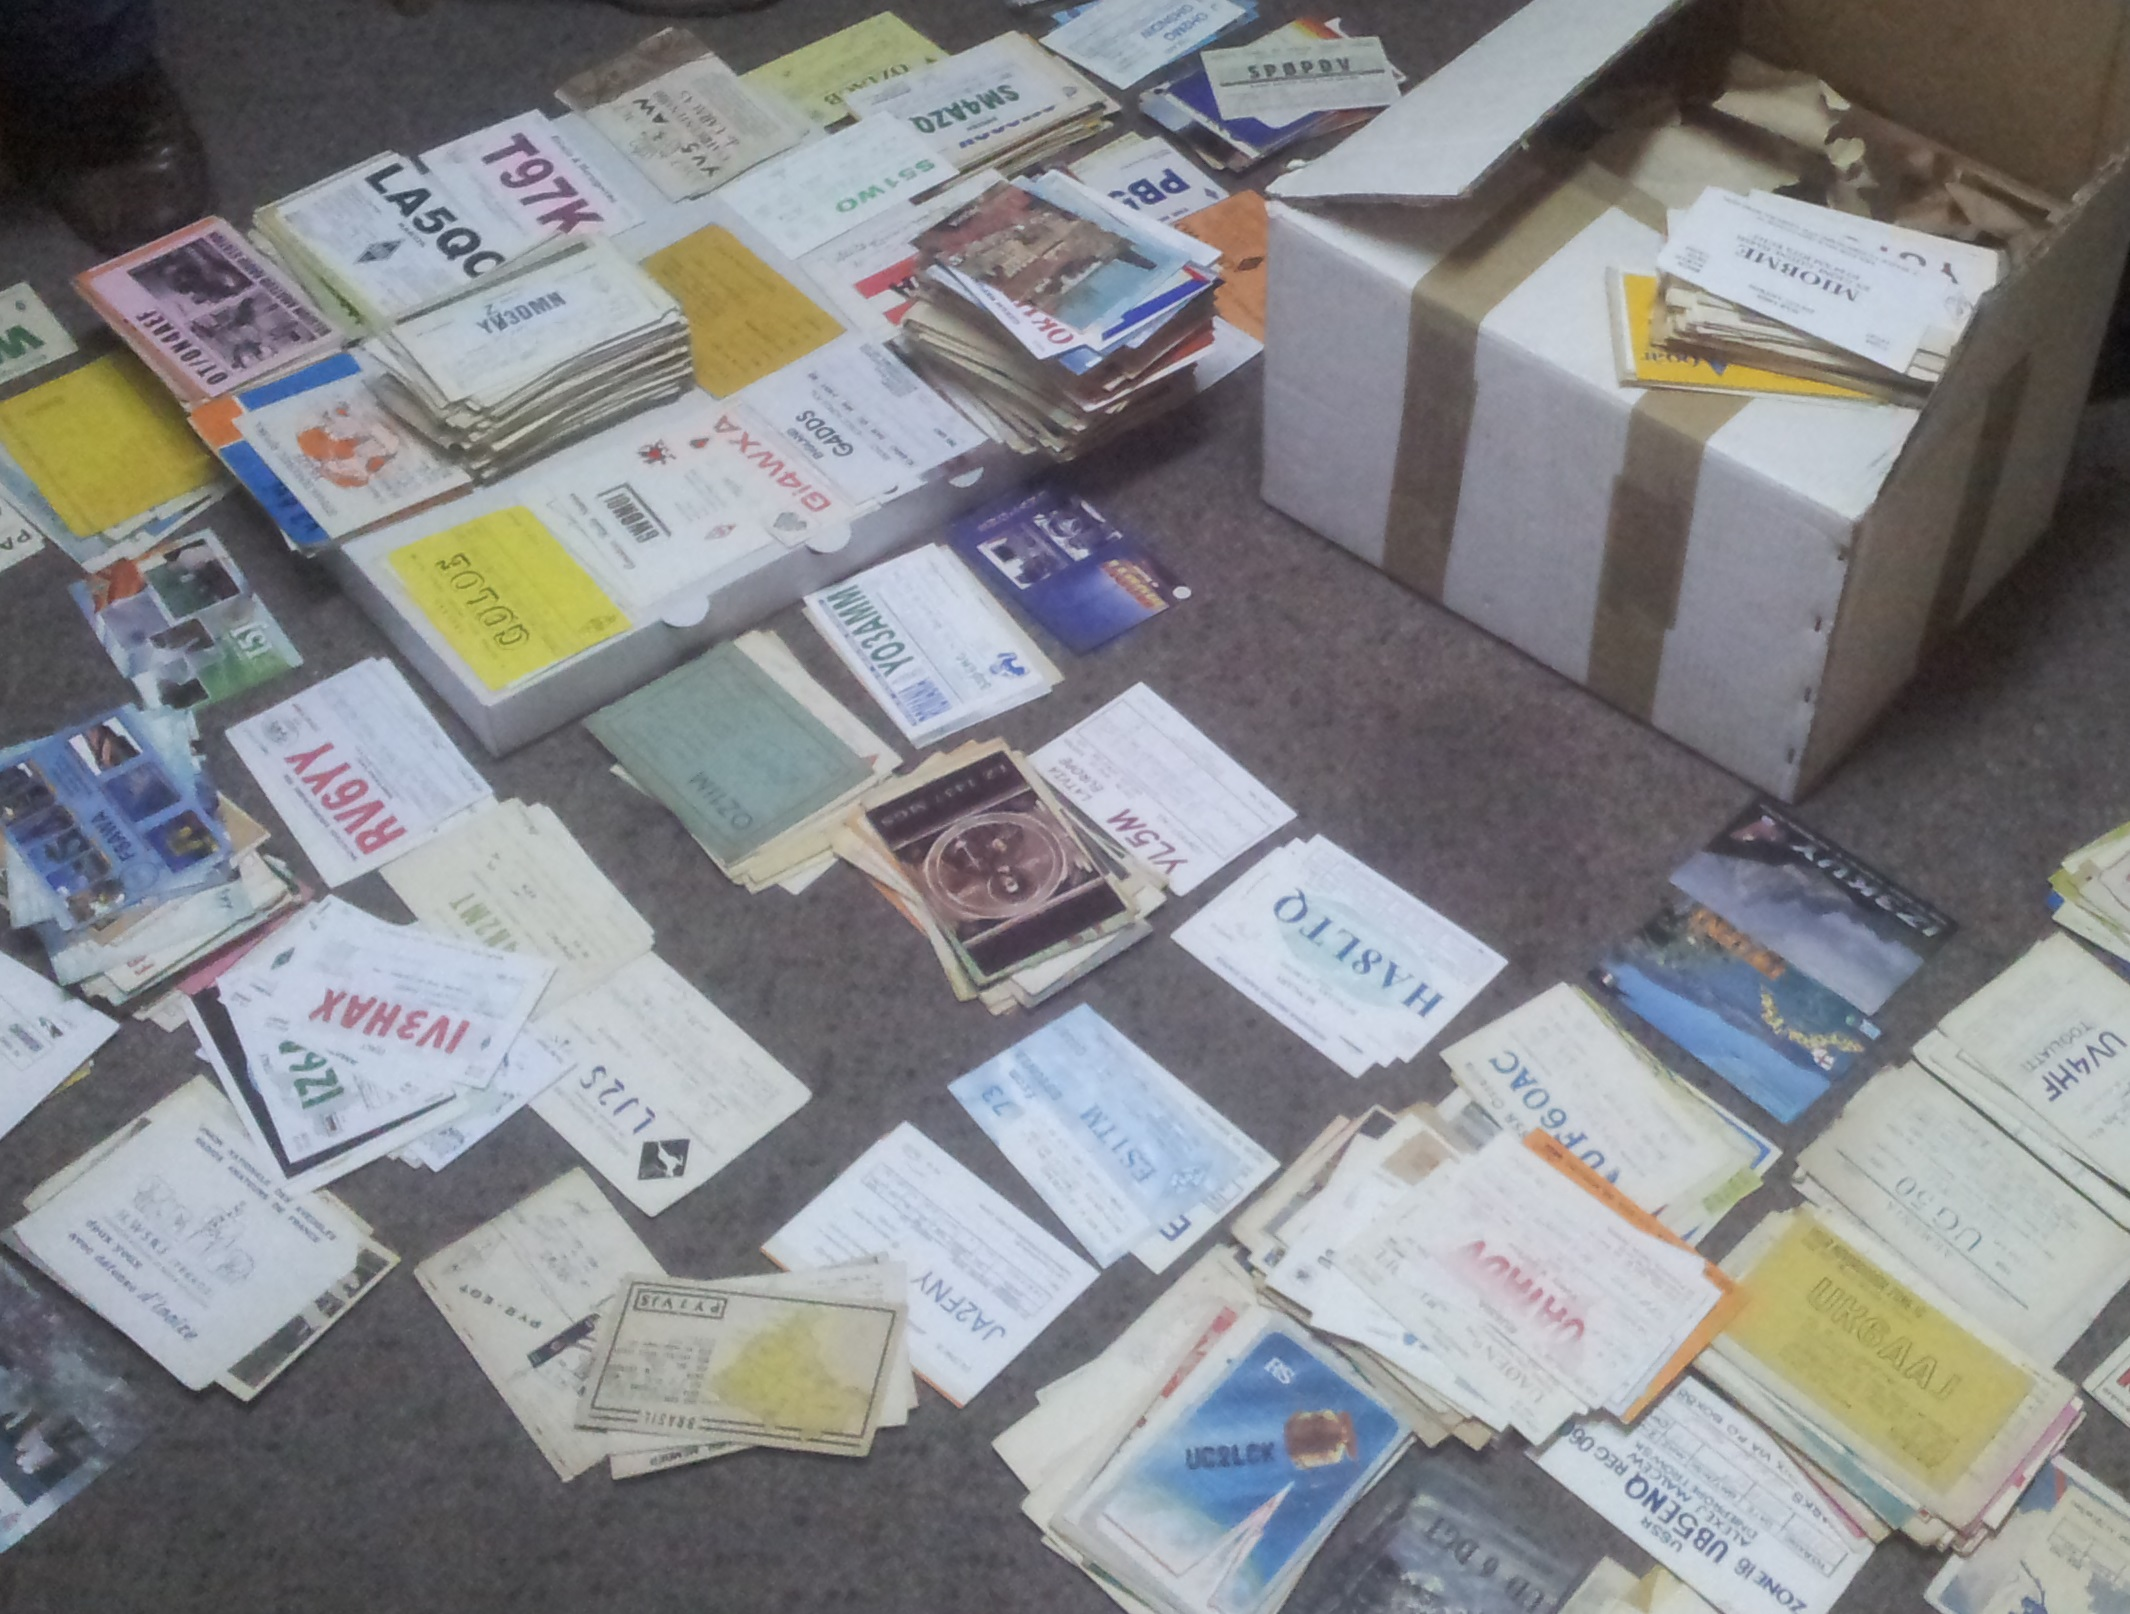
\includegraphics[width=0.5\textwidth]{qsl_mess}
            \end{center}
            \vspace{-20pt}
            \caption{Duża liczba kart może w pewnym momencie przerodzić się w trudny do opanowania bałagan}
            \vspace{-10pt}
            \label{fig:qsl_mess}
        \end{wrapfigure}
        Po pewnym czasie pracy radioamatora kolekcjonującego kraje powstają pewne problemy. Liczba krajów, z którymi przerowadzono łączność, rośnie początkowo bardzo szybko i na pewnym etapie trudno pamiętać, które kraje zostały już ,,zrobione''. Sugerowanie się samymi kartami QSL też nie jest najlepszym pomysłem. Radioamator pracujący samodzielnie dostanie mało takich kart, chyba że będzie korzystał z usług biura QSL. Z kolei liczba łączności przeprowadzonych przez stacje klubowe może dojść do tak dużych wielkości, że nadzór nad historią może stać się niemożliwy. Na rysunku \ref{fig:qsl_mess} można zobaczyć próbę porządkowania starych kart QSL przez członków klubu krótkofalowców SP6PWT.

        Konieczne w takiej sytuacji jest prowadzenie \textbf{logu krótkofalarskiego} - specjalnego dziennika, w którym zapisywane są wszystkie szczegóły przeprowadzonych łączności - czas, znak rozmówcy, raporty RST, a nawet imię i nazwisko rozmówcy oraz jego adres. Początkowo takie dzienniki prowadzone były na papierze. Doświadczeni krótkofalowcy posiadali bogate dzienniki łączności zawierające po kilka tysięcy wpisów. Wraz z nadejściem ery komputerów papierowe dzienniki można było zastąpić komputerowymi programami do logowania łącznośći (tzw. Loggery). Dzięki nim znacznie prostsze jest późniejsze wyszukiwanie łączności wg. kryteriów. Przykładem takiego komputerowego logu może być nawet serwis internetowy qrz.com (której podstawowym zadaniem jest możliwość obejrzenia profilu użytkownika identyfikującego się znakiem wywoławczym). W nim możemy na bierząco dodawać nowe łączności lub zmieniać szczegóły poprzednio stworzonych. Dodawać łączności do bazy można także poprzez import pliku w odpowiednim formacie, wygenerowanego z programu komputerowego. Najbardziej popularnym formatem eksportu zbioru łączności jest format \textbf{ADIF}\footnote{ADIF (ang. Amateur Data Interchange Format)} opisany w podpunkcie \ref{sec:adif}. Gotowy plik w formacie ADIF można importować w serwisie qrz.com i w ten sposób dodać na raz wszystkie swoje łączności zapisane w lokalnym programie komputerowym. Istnieje także możliwość eksportu danych w formacie ADIF z serwisu qrz.com, lecz konieczne do tego jest zapłacenie za rozszerzenie możliwości konta.
            \subsection{Format ADIF}
            \label{sec:adif}
            ADIF to otwarty standard wymiany danych pomiędzy programami używanymi przez radioamatorów. Został stworzony w odpowiedzi na potrzeby krótkofalowców, którym doskwierały problemy związane z koniecznością konwertowania danych przenoszonych pomiędzy używanymi przez nich programamami. Zaraz po opracowaniu został zaimplementowany w większości popularnych programach dla krótkofalowców. Jest nieskończenie rozszerzalny. Może przenosić dane zarówno binarne jak i tekstowe. Nowe dane mogą być dodawane bez zmiany struktury starych danych. Jest łatwy w implementacji we wszystkich popularnych językach programowania. Dane same w sobie są łatwe do odczytania gołym okiem w pliku - struktura danych w pliku jest spójna i czytelna.

            Standard ADIF nie ogranicza się tylko do przechowywania i przesyłania wpisów dziennika łączności. Może przekazywać takie dane jak np. zasady zawodów i musi być gotowy na przyjęcie kolejnych typów danych w związku z tym, że hobby cały czas ewoluuje.

            Na standard ADIF składają się 4 komponenty:
            \begin{description}
                \item[Specyfikacja fizyczna] - Jak mają być zapisywane pola i rekordy w pliku.

                Każde pole musi być poprzedzone nazwą pola oraz długością zapisanej danej otoczonymi nawiasami ostrokątnymi < i >. Nazwa i długość rozdzielone są dwukropkiem. Nazwa może być zapisana wielkimi literami, małymi literami lub w dowolnej kombinacji. Jest to bez znaczenia. Długość pola wartości oznacza liczbę znaków ASCII i może przyjąć dowolną niezerową wartość. Przykładowe pole oznaczające znak wywoławczy rozmówcy: \texttt{<CALL:6>WN4AZY}. 

                Krotki tworzone są z wielu pól i zakończone są znacznikiem \texttt{<EOR>}\footnote{EOR (ang. End-Of-Record)}. Na przykład: \texttt{<CALL:6>WN4AZY<BAND:3>20M<QSO\_DATE:8>19960513<TIME\_ON:4>1305<EOR>}.

                Przed właściwymi danymi można załączyć nagłówek w którym można dodać informacje o wersji standardu, z jakiego programu zostały wyeksportowane dane itd. Nagłówek musi zaczynać się od znaku innego niż '\texttt{<}' i zostać zakończony znacznikiem \texttt{<EOH>}\footnote{EOH (ang. End-Of-Header)}

                Ważną kwestią jest to, że w obszarze wartości pola może być dowolna liczba znaków, jednak branych pod uwagę jest tylko tyle ile określonych jest w obszarze długości. Po znaczących danych mogą być jeszcze dowolne komentarze, znaki nowej linii itp. Program importujący po odczytaniu obszaru wartości na podstawie określonej długości musi odczytywać kolejne znaki (ignorując je) aż do momentu, gdy natrafi na znak '\texttt{<}' rozpoczynający kolejne pole lub znacznik \texttt{<EOR>} kończący odczytywaną krotkę.

                Nie ma żadnej specyfikacji dotyczącej kolejności pól w krotce. Mogą się one pojawić w dowolnej kolejności. Nieustawione pola zostaną pominięte przy tworzeniu obiektu w bazie danych podczas importu pliku, więc obiekty w bazie danych mogą mieć różne pola. Specyfikacja nie zabrania także pól o zerowej długości, więc programista w tworzonej aplikacji powinien przewidzieć taką ewentualność. Podane przykłady pokazane zostały z użyciem znaków \textbf{ASCII}, lecz specyfikacja pozwala na dowolny typ danych oraz dowolną długość danych. Format ADIF może zostać wykorzystany na przykład do przesyłania obrazów lub dokumentów tekstowych. 
                \item[Definicje typów pól] - Jak konkretny typ danych ma być zapisany w pliku. Dla przykładu data (pole \textbf{DATE}) powinno być zapisane przy pomocy znaków \textbf{ASCII} w~formacie \textbf{YYYYMMDD}.
                \item[Definicje pól] - Lista elementów (znak wywoławczy, data, jednostka DXCC itd.) i opis poprawnych wartości w ich polach. Każde pole ma nazwę, która składa się z od 1~do 10 znaków. Możliwymi znakami w nazwie pola są: \textbf{A}-\textbf{Z}, \textbf{0}-\textbf{9} oraz '\_', lecz nazwa musi zaczynać się literą. Na przykład dla pola \textbf{CONT} oznaczającego kontynent poprawnymi wartościami są tylko: \textbf{NA}, \textbf{SA}, \textbf{EU}, \textbf{AF}, \textbf{OC} i \textbf{AS}.
                \item[Definicje plików] - Opis kategorii danych. Na przykład plik \textbf{Logu} jest określany jako wszystkie dane konieczne do zaliczenia łączności (znak wywoławczy rozmówcy, data łączności, pasmo i modulacja) oraz wszystkie informacje uzupełniające (komentarze, punktacja w zawodach, imię korespondenta itd.). Każde dodatkowe pole (spoza kategorii) może być dołączone do pliku, lecz nigdy nie ma gwarancji, że wartości z~tego pola zostaną zaimportowane przez docelowy program.
            \end{description}

        \section{DX Cluster}
        \label{sec:dxcluster}
        Praca radioamatora opiera się na poszukiwaniach. Polega na przeszukiwaniu częstotliwości w celu znalezienia ciekawych i odległych stacji. Nie da się jednak siedzieć przy radioodbiorniku przez cały czas. A nawet jeśli by się dało, to przeszukiwanie wszystkich dostępnych częstotliwości na okrągło jest bardzo monotonne. Dobrym pomysłem jest wzajemnie informowanie się przez krótkofalowców. W tym właśnie pomagają komputerowe serwisy DX Cluster. Kiedy radioamator przeprowadzi łączność ze stacją z rzadko spotykanej jednostki DXCC lub inną ciekawą stacją (znak okolicznościowy, wyprawa krótkofalarska), może poinformować o tym swoich kolegów. Po podłączeniu do serwisu DX Cluster (najczęściej protokołem Telnet, lecz ostatnio często przez interfejs WWW) publikuje się infirmację \textbf{KTO}, \textbf{Z KIM}, \textbf{KIEDY} i \textbf{GDZIE} (częstotliwość) przeprowadził wartą uwagi łączność. Jest to tak zwany \textbf{Spot DX}. 

        Użytkownicy podłączeni do DX Clustera mają możliwość publikowania ogłoszeń o~spotach DX i odpowiadania na ogłoszenia, wysłania prywatnych komunikatów do innych użytkowników, wysyłania i odbierania poczty, wyszukiwania i odbierania danych archiwalnych i dostępu do informacji zgromadzonych w bazach danych.

        Każdy z DX Clusterów jest inny. Każdy jest prowadzony przez innego krótkofalowca, przez grupę lub klub. Przez to DX Clustery mają różne możliwości. Obsługa tego typu serwisu, zwłaszcza przez protokół Telnet, jest dość mało intuicyjna. Po podłączeniu do Clustera należy się do niego zalogować swoim prywatnym znakiem wywoławczym. Niektóre serwisy proszą o potwierdzenie logowania hasłem. Po zalogowaniu serwis wysyła powitanie i pokazuje najważniejsze komendy obsługi. Z racji tego, że większość komend jest mało intuicyjna, autorzy przygotowują obszerne dokumentacje i instrukcje obsługi. Ważną rzeczą jest to, że nie trzeba odwiedzać wszystkich istniejących Clusterów aby mieć dostęp do wszystkich wysyłanych komunikatów. Wszystkie największe Clustery synchronizują się między sobą przekazując sobie na bieżąco najnowsze spoty.

        Wiadomości o spotach jakie można otrzymać mają swoją ściśle zdefiniowaną strukturę opisaną na poniższym przykładzie:

        \noindent\texttt{DX\space de\space IQ5WT:\space\space\space\space\space 7179.0\space\space IZ5GST/P\space\space\space\space\space DCI-PI149 WCA13234\space\space\space\space\space\space\space\space 0735Z\space FN42}

        \begin{description}
            \item[Znaki 1-5] - Kombinacja liter 'DX de ' oznaczająca początek spotu oraz to, że następnymi znakami będzie znak wywoławczy spottera (autora spotu).
            \item[Znaki 7-13] - Znak wywoławczy autora spotu.
            \item[Znaki 15-24] - Częstotliwość (podana w kHz z jedną cyfrą dziesiętną oddzieloną kropką), na której przeprowadzona została łączność.
            \item[Znaki 26-38] - Znak wywoławczy spotowanej stacji - rozmówcy.
            \item[Znaki 40-69] - Dowolny (opcjonalny) komentarz od spottera. Najczęściej umieszczane są tam informacje na temat wykorzystanej modulacji, wymienione raporty RST lub pozdrowienia.
            \item[Znaki 71-75] - Czas przeprowadzonej łączności w formacie UTC (zapis 4-znakowy, format 24-godzinny) zakończony literą Z.
            \item[Znaki 77-80] - Lokator spottera - 4 z 6 znaków.
        \end{description}

        Oprócz spotów za pomocą DX Clustera przesyłane są ogłoszenia (komunikaty). Zwykle są to osobiste wiadomości krótkofalowców do wiadomości wszystkich podłączonych użytkowników lub komunikaty od stacji \texttt{DK$\emptyset$WCY} związane z warunkami propagacyjnymi (aktywność słoneczna i magnetyczna).

        \section{Koncepcja projektu}
        \label{sec:problem_description}
        Ciekawym problemem do rozwiązania może być ułatwienie pracy radioamatorom kolekcjonującym potwierdzone łączności z różnymi krajami oraz chcącym zdobywać różne dyplomy za osiągnięcia z tej dziedziny hobby. Rozwiązaniem tego problemu może być system ekspertowy bazujący na bazie danych i informacjach odczytywanych z systemu DX Cluster, aby pokazać radioamatorowi specjalnie dla niego przydatne informacje.

        Głównymi założeniami tego projektu powinny być: wysoka mobilność całego systemu, zgodność ze standardem plików ADIF oraz prostota i intuicyjność obsługi systemu przez użytkowników.

    \chapter{Przegląd dostępnych rozwiązań}
    \label{sec:existing_possibilities}
    Rozdział ten prezentuje różne możliwości realizacji projektu podzielone na jego główne składniki i porównuje je pod kątem jego założeń. Na wstępie należy zaznaczyć, że do tworzenia projektu wybrany został język Python ze względu na jego wysoką czytelność oraz duże wsparcie programowania zorientowanego obiektowo. Na końcu rozdziału zostanie przedstrawione podsumowanie, w którym zostanie wybrany komplet komponentów i~rozwiązań, które będą stanowić podstawę projektu.

        \section{Obsługa systemu DX Cluster}
        \begin{figure}[hb]
            \centering
            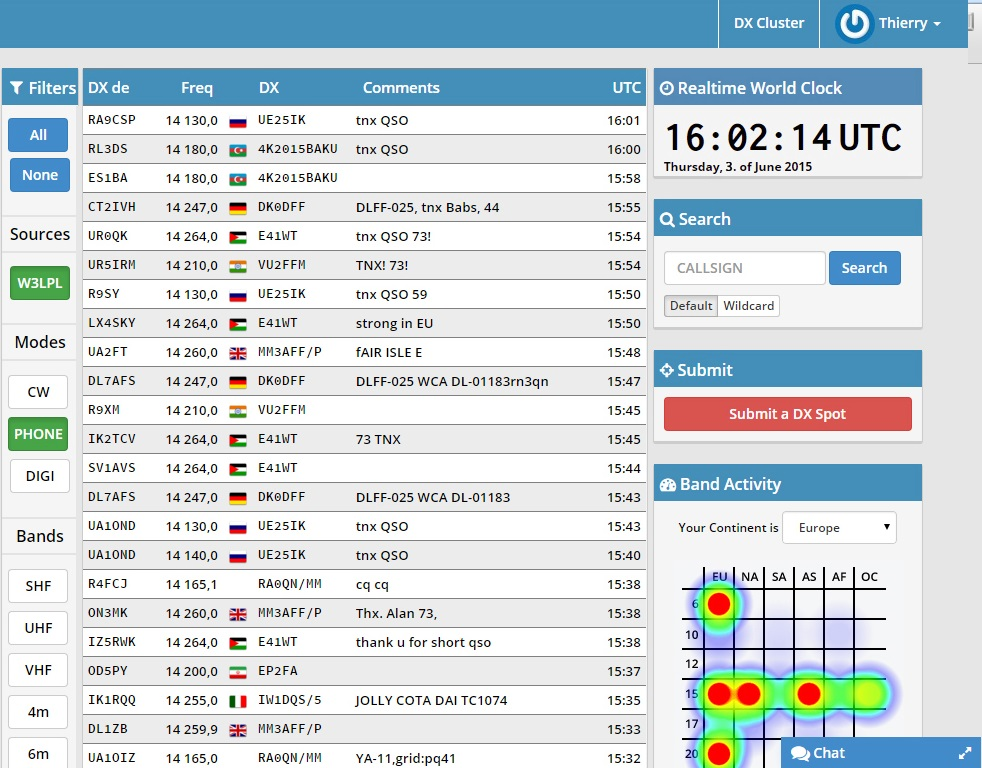
\includegraphics[width=0.8\textwidth]{dxheat}
            \caption{DX HEAT - Przykładowy DX Cluster z interfejsem WWW.}
            \label{fig:dxheat}
        \end{figure}

        Pierwszym elementem systemu jest zewnętrzny system DX Cluster, do którego będzie można się podłączyć i czytać z niego przesyłane przez innych użytkowników dane. DX Cluster można obsługiwać na dwa sposoby - poprzez protokół Telnet, gdzie do systemu należy się uprzednio zalogować i odpowiednio czytać dane lub wprowadzać do niego komendy. Drugim sposobem pozyskiwania informacji z systemu DX Cluster jest interfejs WWW. Wiele właścicieli Clusterów zaprojektowało estetyczne i czytelne strony internetowe, gdzie prezentowane są dane z Clustera. Przedstawiony na rysunku~\ref{fig:dxheat} to jeden najpopularniejszych publicznie dostępnych Clusterów z interfejsem WWW. Pozwala on na filtrację spotów na podstawie \textbf{modulacji}, \textbf{pasma}, oraz \textbf{kontynentów - swojego i poszukiwanego}. Przedstawia także dwa najpotrzebniejsze wskaźniki dotyczące stanu zakłóceń słonecznych i magnetycznych, które mają znaczący wpływ na jakość propagacji. W bardzo przejrzysty sposób prezentuje także ,,ruch'' na różnych pasmach w zależności od poszukiwanego kontunentu. Oczywiście jeżeli system ma działać automatycznie, wtedy lepiej przygotować go do czytania danych ze źródła przeznaczonego do tego celu - za pomocą protokołu Telnet. Odczytywanie strony WWW, która ma w sobie wiele dynamicznych elementów JavaScript i dane odświeżane za pomocą techniki AJAX nie jest rozsądnym wyborem. Ciągłe odświeżanie strony a następnie parsowanie danych jest niepotrzebną pracą w porównaniu do prostego odczytywania kolejnych linii znaków przesyłanych do klienta Telnet. Kolejny wybór pada na konkretny DX Cluster. Obecnie oficjalnych DX Clusterów działa ponad kilkadziesiąt, więc wybór jest duży. Priorytetami przy wyborze Clustera były:

        \begin{itemize}
            \item Wysoka niezawodność
            \item Proste logowanie
            \item Mała konieczność interakcji z samym Clusterem
        \end{itemize}
        \begin{wrapfigure}{r}{0.5\textwidth}
            \vspace{-25pt}
            \begin{center}
                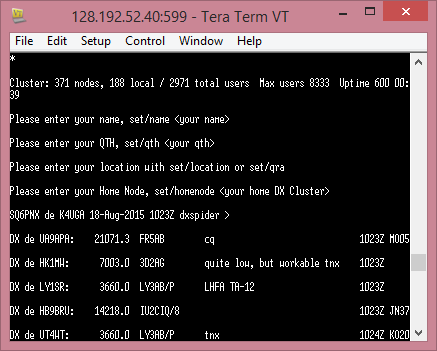
\includegraphics[width=0.40\textwidth]{k4uga}
            \end{center}
            \vspace{-20pt}
            \caption{Klient Telnet podłączony do Clustera \texttt{K4UGA}}
            \vspace{-20pt}
            \label{fig:k4uga}
        \end{wrapfigure}

        Wybór padł na Cluster \texttt{K4UGA} działający w Stanach Zjednoczonych w stanie Georgia. Jest on jednym z najbardziej niezawodnych obecnie działających Clusterów. Logowanie polega na wpisaniu swojego znaku wywoławczego (nie trzeba podawać hasła dostępu) a potem nie są wymagane już żadne działania, Cluster od razu przesyła najnowsze spoty, co widoczne jest na rysunku~\ref{fig:k4uga}.

        Do połączenia poprzez protokół Telnet została stworzona bardzo wygodna biblioteka w języku Python o nazwie \texttt{telnetlib}.

        \section{Format plików dziennika}
        Format plików jaki będzie przetwarzany już został wybrany i będzie nim format \textbf{ADIF}. Wybór był oczywisty - jest to format niezaprzeczalnie najpopularniejszy i wykorzystany w większości oprogramowania do zastosowań krótkofalarskich. Warto jednak przedstawić ten format na tle innych, także bardzo popularnych formatów plików.

            \subsection{ADIF}
            Format ADIF został już omówiony w rozdziale~\ref{sec:adif}. Jego największymi atutami jest, to że jest otwartym standardem i został stworzony przez krótkofalowców dla krótkofalowców. Jest na tyle rozpowszechniony i używany, że można założyć, że jest formatem najbardziej uniwersalnym. Dodatkowymi założeniami polityki standardu ADIF są: kompatybilność wprzód (plik ADIF zgodny z jedną wersją standardu będzie poprawnie odczytany przez oprogramowanie zgodne z tą samą lub nowszą wersją standardu); zgodność z wycofanymi polami (pola przestarzałe i wycofane z użytku muszą być akceptowane przy imporcie plików ADIF przez oprogramowanie, ale nie powinny być generowane przy eksporcie pliku w tym formacie).

            \subsection{ADX - XML ADIF}
            Dodany do standardu ADIF w najnowszej wersji 3.*, nowy format pliku oparty o składnię \textbf{XML}. Ma to swój cel we wsparciu międzynarodowych typów danych używających znaków Unicode zakodowanych w systemie UTF-8. Po wprowadzeniu formatu \textbf{ADX}, format ADIF został przemianowany na \textbf{ADI}.

            Struktura pliku ADX jest bardziej usystematyzowana niż w pliku ADI ze względu na użycie łatwych do przetwarzania znaczników XML. Plik ADX składa się z kilku części. Pierwsza część to jednolinijkowy nagłówek XML określający zgodność z wersją XML oraz zastosowane kodowanie znaków.

            \noindent Na przykład: \texttt{<?xml version="1.0" encoding="UTF-8"?>}.

            \noindent Po nagłówku xml jest zapisany cały plik w formacie ADX i jest musi być otoczony znacznikami \texttt{<ADX>} i \texttt{</ADX>}. Następnie podobnie jak w~formacie ADI można zapisać kilka istotnych danych dla samego pliku w nagłówku ADX. Cały nagłówek ADX mieści się pomiędzy znacznikami \texttt{<HEADER>} i \texttt{</HEADER>}. Każdy z~wpisów nagłówka zawarty jest pomiędzy znacznikami \texttt{<nazwa\_pola>} i \texttt{</nazwa\_pola>}. Po sekcji nagłówka rozpoczyna się sekcja danych i jest ona otoczona znacznikami \texttt{<RECORDS>} i \texttt{</RECORDS>}. Każda krotka w pliku mieści się pomiędzy znacznikami \texttt{<RECORD>} oraz \texttt{</RECORD>} i podobnie jak w sekcji nagłówka, każde pole z wartością zawarte jest pomiędzy znacznikami \texttt{<nazwa\_pola>} i~\texttt{</nazwa\_pola>}. Przykładowy plik ADX został przedstawiony poniżej:

            \lstinputlisting[language=Xml, frame=single, caption=Prosty przykład pliku ADX]{sample_adx.xml}

            \subsection{Cabrillo}
            Drugi najpopularniejszy format zapisu logów krótkofalarskich, lecz wykorzystywany praktycznie \underline{tylko w zawodach}. Do niedawna powszechnym było stosowanie ręcznie wypełnianych (papierowych) formularzy logów z zawodów. Wraz z upowszechnieniem komputerów zaczęto wykorzystywać tę technologię i wprowadzano wydruki papierowe, wyniki przesyłane na dyskietkach i od kilkunastu lat wysyłkę logów pocztą elektroniczną. Wprowadzenie komputerów znacznie ułatwiło startującym pracę w zawodach i skróciło do minimum najnudniejszą część zawodów, czyli wypełnianie dzienników. Niestety nie było to takie dobre dla komisji zawodów. Przeszkodą był brak standardu plików przesyłanych przez użytkowników zawodów. Wynikało to z tego, że oprogramowanie logujące pracę w zawodach było pisane przez różnych autorów, a co za tym idzie każdy autor przyjmował swój własny standard zapisu logów do pliku. Przyczyniało się to do tego, że praktycznie niemożliwym było napisanie oprogramowania rozliczającego zawody. Rozwiązaniem tego problemu miał być format Cabrillo stworzony około roku 1999. Uczestnicy zawodów mogą korzystać z~dowolnego programu do logowania łączności, pod warunkiem, że potrafi on eksportować dane w formacie Cabrillo. W pliku znajdują się wszystkie niezbędne informacje o przeprowadzonych łącznościach i dane dodatkowe. Minusem formatu Cabrillo jest to, że nie jest on uniwersalny i ma bardzo ścisłą strukturę znaków. Prowadzi to do tego, że każdy organizator zawodów powinien opracować własną odmianę formatu Cabrillo w zależności od regulaminu prowadzonych zawodów. Po opracowaniu tego rozwiązania powinien on zostać rozpowszechniony wśród autorów programów logujących.

            Sam plik rozpoczyna się znacznikiem \texttt{START-OF-LOG} numerem wersji formatu Cabrillo i kończyć znacznikiem \texttt{END-OF-LOG}. Wewnątrz, składa się z dwóch części: nagłówka i~danych o przeprowadzonych łącznościach. W nagłówku powinny zostać zawarte wszystkie niezbędne dane określone przez organizatora zawodów. Zwykle są to:
            \begin{itemize}
                \item Znak wywoławczy
                \item Nazwa zawodów
                \item Kategoria zawodów
                \item Nazwa klubu, do którego ma być doliczony wynik zgłaszającego
                \item Dane teleadresowe uczestnika
                \item Informacje o sprzęcie i oprogramowaniu
                \item Deklarowana suma zdobytych punktów - może zostać pominięta, ponieważ oprogramowanie rozliczające zawody będą wyliczały wynik na podstawie przesłanych wszystkich logów.
            \end{itemize}
            Druga część pliku to właściwy log. Składa się on z kolejno ułożonych wpisów, gdzie każdy jeden wpis to kolejna łączność (każdy wpis w kolejnej linii). Dane w każdym polu są ściśle ustawione na swoich pozycjach. Dla przykładu znak korespondenta może rozpoczynać się na 56 znaku, a kończyć na 68 znaku każdej linii. Umieszczenie danych w niewłaściwej kolejności lub złe wyrównanie znaków spowoduje błędne odczytanie zawartych informacji i nie zaliczenie łączności.

        \section[Web Framework]{Web Framework\footnote{Framework lub platforma programistyczna - szkielet do budowy aplikacji. Definiuje strukturę aplikacji, a także dostarcza zestaw komponentów i bibliotek ogólnego przeznaczenia do wykonywania określonych zadań. Programista tworzy aplikację rozbudowując i dostosowując poszczególne komponenty do wymagań realizowanego projektu, tworząc w ten sposób gotową aplikację.}}
        Z racji tego, że projekt zakłada komunikację z wieloma użytkownikami jednocześnie oraz wygodną prezentację wyników, należało stworzyć prosty interfejs WWW. Językiem, który został użyty do programowania był \textbf{Python}, więc oczywistym było skorzystanie z~jednego z~kilku dostępnych frameworków. To znacznie skróciło czas tworzenia aplikacji internetowej.

            \subsection{Django}
            Django to framework w całości napisany w języku Python. Opracowany pod koniec 2003 roku doczekał się 8 oficjalnych wersji. Od 2005 roku jest rozpowszechniany na licencji BSD. Jego głównym założeniem jest ułatwienie tworzenia serwisów internetowych, zwłaszcza tych, których podstawą jest baza danych. Stawia duży nacisk na możliwość ponownego użycia komponentów, szybki rozwój aplikacji i głęboko wspiera zasadę DRY\footnote{DRY (ang. Don't Repeat Yourself, Nie Powtarzaj Się) - reguła zalecająca unikanie różnego rodzaju powtórzeń. Unikanie tych samych (lub bardzo podobnych) fragmentów kodu w wielu miejscach. Powtarzający się kod można zapisać jako oddzielną funkcję i odwoływać się tylko do niej znacząco zwiększając czytelność kodu. Metoda poprawnie zastosowana przynosi znaczną oszczędność czasu zarówno przy poszukiwaniu błędów jak i przy nanoszeniu poprawek (bład trzeba poprawić tylko w jednym miejscu).}. Język Python jest w Django używany praktycznie do wszystkiego, włącznie z ustawianiem parametrów, plików i definiowaniem modeli danych.

            Opiera się na wzorcu projektowym Model-View-Controller (Model-Widok-Kontroler). Model jest reprezentacją problemu bądź logiki aplikacji. Odpowiada za odwzorowanie obiektów w strukturze bazy danych i ich relacje. Widok jest opisem wyświetlania pewnej części modelu. Służy do tworzenia zapytań, filtrowania, szeregowania i agregacji danych. Kontroler przyjmuje dane wejściowe od użytkownika i reaguje na jego poczynania, zarządzając aktualizację modelu i odświeżenie widoków.

            Popularne jest także określenie frameworka Django jako pracującego w formie Model-View-Template (Model-Widok-Szablon). Szablon to graficzny opis struktury strony internetowej. Definiuje gdzie ma się znaleźć jaki element (zwykle tworzony w języku HTML z~odpowienimi wstawkami).

            Jego najważniejszymi zaletami są:
            \begin{itemize}
                \item Bogata i przyjazna dla programistów dokumentacja
                \item Ogromna społeczność wspierająca pracę nad projektem i służąca pomocą niedoświadczonym programistom
                \item Wbudowany serwer WWW służący do szybkiego testowania aplikacji
                \item Automatycznie generowany i kompletny panel administracyjny z możliwością dalszego dostosowania do potrzeb użytkowników
                \item Prosty i funkcjonalny system szablonów czytelny zarówno dla grafików jak i programistów
                \item Wsparcie dla wielojęzycznych aplikacji
                \item Bardzo duża skalowalność i wydajność pod obciążeniem
                \item Obsługa baz danych MySQL, PostgreSQL, SQLite oraz Oracle
            \end{itemize}

            Używany przez takie popularne serwisy jak \textbf{Instagram}, \textbf{The Washington Times}, \textbf{Bitbucket} czy \textbf{Pinterest}.

            \subsection{Flask}
            Flask to mikroframework do Pythona na licencji BSD. Początkowo został stworzony jako żart prima-aprilisowy, który miał udowodnić, żę można stworzyć framework zawierający się w jednym pliku. W przeciwieństwie do Django nie zapewnia żadnego szkieletu ani podstawy dla tworzonej aplikacji. Nie zawiera gotowych rozwiązań i wbudowanych komponentów. Nie zawiera panelu admina. Ma jednak bogate zaplecze dodatków i rozszerzeń, które można bez problemu dołączać do projektu. Głównie przeznaczony jest do małych, prostych projektów, które wymagają aplikacji opartych o jedną lub dwie funkcje.

            W porównaniu do Django:
            \begin{itemize}
                \item Ma równie bogatą, lecz mało uporządkowaną dokumentację
                \item Nauka pracy z tym frameworkiem polega na studiowaniu tutoriali a nie czytaniu dokumentacji
                \item Sam z siebie jest bardzo ubogi - jego siła tkwi w możliwych do doinstalowania dodatkach
                \item W przeciwieństwie do Django dużo częściej wykorzystywany jest do tworzenia prostych projektów
                \item Nie ma możliwości mapowania relacyjno-obiektowe - programista sam musi pisać zapytania do wykorzystywanej bazy danych, w Django wystarczyć stworzyć obiekt lub wykonać na tym obiekcie jakąś metodę, a zapytanie do bazy generuje się samo.
            \end{itemize}

            Frameworka Flask używa popularny serwis \textbf{LinkedIn}.

            \subsection{Pylons}
            Pylons to lekki framework napisany w języku Python, który czerpie najlepsze rozwiązania z języków Ruby, Python i Perl. Jest przez wielu uważany za główną alternatywę dla Django. Umożliwia tworzenie bardzo elastycznych i skalowalnych projektów aplikacji internetowych. Był jednym z pierwszych projektów adaptujących standard WSGI umożliwiający wielokrotne wykorzystanie komponentów lub nawet całych aplikacji w wielu projektach. W swojej budowie jest zbliżony do stworzonego w języku Ruby frameworka Ruby on Rails. Jego pierwotnym założeniem jest tworzenie aplikacji szybko, elastycznie i~prosto.

            W porównaniu do Django:
            \begin{itemize}
                \item Doskonałe wsparcie dla techniki Ajax. Django do tej pory nie posiada wbudowanej implementacji Ajax'a.
                \item Uboga dokumentacja.
                \item Bardziej uciążliwe korzystanie z formularzy.
                \item Mapowanie relacyjno-obiektowe oparte o manager SQLObject. Django korzysta z~własnego mapera relacyjno-obiektowego. Ma dużo bardziej elegancką składnię i~lepszą dokumentację.
                \item Brak wbudowanego panelu administracyjnego - wizytówką Django jest panel administracyjny gdzie praktycznie z miejsca można zarządzać całą swoją zaprojektowaną bazą danych (Dodawać, usuwać, modyfikować obiekty w bazie). We frameworku Pylons panel admina pozostawia dużo do życzenia.
            \end{itemize}

            \subsection{Pyramid}
            Pyramid to framework stworzony jako odnoga projektu Pylons. Używany jest jako ,,gotowy do działania'', lecz nie zakłada z miejsca z jakich komponentów ma korzystać.

            Społeczność korzystająca i wspierająca Pyramid rośnie z dnia na dzień. Ogromną zaletą jest także profesjonalna dokumentacja, która w założeniu ma być tak dobra, aby uniknąć wsparcia ze strony społeczności. Głównymi założeniami tego projektu są minimalizm, szybkość i niezawodność. Jest jednym z pierwszych frameworków kompatybilnych z językiem Python 3.

            W porównaniu do Django:
            \begin{itemize}
                \item Wsparcie dla Ajax
                \item Elastyczność przy budowaniu aplikacji - każdy komponent może być włączony i~wyłączony w każdej chwili, każdy problem może być rozwiązany na kilka alternatywnych sposobów, można wykorzystać kilka różnych sposobów podłączenia do bazy danych, a nawet można podłączyć serwis do kilku baz danych.
                \item Brak panelu administracyjnego
            \end{itemize}

        \section{Wybór komponentów projektu}
        Jak już zostało wspomniane projekt zakłada użycie w znaczącej części języka Python (oczywiście z pominięciem języka HTML i CSS do stworzenia interfejsu graficznego strony WWW).

        Po przeanalizowaniu możliwości wykonania projektu i biorąc pod uwagę wszystkie założenia projekt będą charakteryzować:
        \begin{itemize}
            \item Obsługa systemu DX Cluster poprzez protokół Telnet. Jest to oczywisty wybór z~racji tego, że w ten sposób otrzymujemy od systemu suche dane, które po mało obciążającej obróbce są gotowe do przetwarzania.
            \item ADIF jako obsługiwany format plików dziennika (logu krótkofalarskiego). Chociaż nie jest tak uniwersalny i łatwy i przetwarzaniu jak formaty oparte o XML, to jest to format najbardziej rozpowszechniony w środowisku któtkofalarskim.
            \item Wybór Web Frameworka padł na Django. Choć jest dużo potężniejszy niż inne rozwiązania dostępne na rynku, to ma ogromną dokumentację i wsparcie społeczności, a także mnogość wbudowanych komponentów. To będzie przekładać się na tworzenie dobrej jakości kodu, sprawdzonych rozwiązań i łatwość rozbudowie już istniejącego systemu.
        \end{itemize}

    \chapter{Realizacja projektu}
    \label{sec:project_realization}
    Praca nad projektem składała się z kilku luźno powiązanych ze sobą etapów. Pierwszym etapem było przygotowanie systemu operacyjnego, bazy danych oraz instalacja frameworka Django. Następnie koniecznym było przygotowanie programu odczytującego dane z systemu DX Cluster za pomocą protokołu Telnet, zapis tych danych do bazy oraz poprawne ustawienie systemu operacyjnego aby w razie restartu program ten uruchomił się samoczynnie. Kolejnym etapem było zaprojektowanie klasy służącej do importowania dzienników w formacie ADIF. To wiązało się także z przygotowaniem w bazie danych tabel z informacjami o jednostkach DXCC i ich prefiksach. Następnie koniecznym było przygotowanie konfigurowalnych profili użytkowników, w których można ustalać to, co jest przez użytkownika poszukiwane. Końcowym etapem było powiązanie potrzeb użytkowników z ich zapisanymi łącznościami oraz z danymi na bieżąco odczytywanymi z systemu DX Cluster.

        \section{Przygotowanie systemu}
        Cały projekt został uruchomiony na systemie operacyjnym GNU/Linux Ubuntu 14.04.2 LTS w wersji serwerowej (bez środowiska graficznego). Interpreter języka Python jest w~systemie wbudowany, więc nie była konieczna jego instalacja. Aplikacja jest oparta na bazie danych SQLite\footnote{SQLite - system zarządzania bazą danych zapisaną w pliku na dysku bez konieczności uruchamiania osobnego procesu bazy danych. Zawartość bazy jest przetrzymywana w jednym pliku binarnym o wielkości maksymalnej 140TB.}, która jest obsługiwana bezpośrednio przez język Python i framework Django, więc nie była konieczna instalacja dodatkowego serwera. Framework Django został zainstalowany w wersji 1.7.7 (najnowszej, stabilnej wersji).

        Po zainstalowaniu oprogramowania i bibliotek Django, należało utworzyć nowy projekt - przestrzeń w której przechowywany będzie kod aplikacji. Zostało to zrobione za pomocą skryptu \texttt{django-admin.py}.

        \texttt{\$ django-admin.py startproject project}\\

        \noindent Django zakłada ścisłą strukturę - projekty, na które składają się poszczególne aplikacje. W obrębie tego projektu została stworzona tylko jedna aplikacja o nazwie \textbf{dx}.

        \texttt{\$ python manage.py startapp dx}\\

        \noindent Istniejący projekt należało skonfigurować w pliku \texttt{project/settings.py}. Wymaganymi ustawieniami były:
        \begin{itemize}
            \item Dodanie aplikacji \textbf{dx} do projektu - Należy do listy \mbox{\textbf{INSTALLED\_APPS}} dodać pozycję 'dx'.
            \clearpage\lstinputlisting[language=Python, firstline=3, lastline=11, frame=single, caption=Dodanie aplikacji \textbf{dx} do projektu]{listings.txt}
            \item Konfiguracja bazy danych - Należy wybrać rodzaj używanej bazy danych (w tym wypadku \texttt{sqlite3}) oraz podać jej nazwę (w przypadku baz SQLite jest to nazwa pliku na dysku.) Te dane muszą zostać przypisane w formie słownika do zmiennej \texttt{DATABASES}. Jak widać na listingu poniżej, plik bazy danych nazywa się \texttt{DXDB.sqlite3} i jest umieszczony w głównym katalogu projektu.
            \lstinputlisting[language=Python, firstline=13, lastline=18, frame=single, caption=Konfiguracja bazy danych]{listings.txt}
            \item Ustawienie języka i strefu czasowej - Te dwie czynności zostały zrealizowane przez przypisanie odpowiednich łańcuchów znaków do zmiennych.
            \lstinputlisting[language=Python, firstline=20, lastline=21, frame=single, caption=Konfiguracja języka i strefy czasowej]{listings.txt}
        \end{itemize}

        \noindent Po zakończonej konfiguracji konieczne jest przeprowadzenia migracji bazy danych (za pierwszym razem równa się to ze stworzeniem pliku bazy na dysku). Migracja przeprowadzana jest poleceniami kolejno:

        \texttt{\$ python manage.py makemigrations}

        \texttt{\$ python manage.py migrate}\\

        W starszych wersjach Django migracja była wywoływana tylko jednym poleceniem, w najnowszej wersji zostało to rodzielone. Ma to swój sens w przypadku korzystania z systemów kontroli wersji. Pobierany jest wówczas tylko plik z zapisanymi szczegółami migracji, nie potrzeba pobierać całego projektu i generować migracji od nowa.

        \section{Pobieranie nowych ,,spotów'' z systemu DX Cluster}
        Cały proces odebrania i zapisania nowego spotu ma kilka kroków, każdy z nich może być rozpatrywany osobno, lecz tworzą one jedną sekwencyjną całość.

            \subsection{Nawiązanie połączenia}
            Pierwszym krokiem jest nawiązanie połącznia z systemem DX Cluster za pomocą protokołu \textbf{Telnet}. Istnieje bardzo wygodna do tego celu biblioteka w języku Python nazwana \texttt{telnetlib}. Dzięki niej można w bardzo prosty sposób stworzyć program, który działa jak klient Telnet.

            Procedura odczytania kolejnych \textbf{spotów} z systemu DX Cluster zawiera kolejne kroki:
            \begin{enumerate}
                \item Otwarcie połączenia protokołem Telnet z odpowiednim adresem IP na konkretnym porcie. W projekcie klient Telnet łączy się z serwerem \textbf{K4UGA} o adresie \texttt{128.192.52.40} na porcie \texttt{599}.
                \item Logowanie do systemu - po podłączeniu system wysyła kilka znaków zachęty do wpisania swojego znaku wywoławczego (na przykład ,,login''). Należy te znaki odczytać a następnie wysłać swój znak wywoławczy (tutaj \texttt{sq6sfs}) wraz ze znakiem powrotu karetki i znakiem nowej linii (\texttt{\textbackslash{}r\textbackslash{}n}).
                \item Po wysłaniu łańcucha znaków ze swoim znakiem wywoławczym należy odczytać to, co system wysyła wzamian. Jeżeli w odpowiedzi znajdzie się słowo ,,invalid'' należy przerwać połączenie i ponowić próbę, ponieważ logowanie nie powiodło się. W projekcie wyrzucony zostaje wyjątek o nazwie \texttt{UsernameError} sygnalizujący problem z procesem logowania do systemu.
                \item Po poprawnym zalogowaniu do systemu, odebrana zostanie wiadomość powitalna oraz informacje szczegółowe o systemie. Dla potrzeb pozyskiwania samych danych o spotach te informacje nie są istotne, więc mogą być pominięte. Ostania linia informacyjna zawiera ciąg \texttt{dxspider} więc do tego momentu wszystko zostaje zignorowane. Następnie należy znaleźć wysłany przez serwer ostatni znak nowej linii przed konkretnymi danymi. Do tego można w wygodny sposób wykorzystać biblioteczne funkcje \texttt{read\_until()}.

                \texttt{self.cluster.read\_until('dxspider')}

                \texttt{self.cluster.read\_until('\textbackslash{}n')}\\
                \item Na tym etapie DX Cluster wysyłać będzie już tylko najnowsze spoty oraz ogłoszenia wysyłane przez innych użytkowników. Pobranie spotu polega na odczytaniu wszystkich znaków do znaku nowej linii.
                \lstinputlisting[language=Python, firstline=24, lastline=31, frame=single, caption=Odczyt nowego spotu]{listings.txt}
                Konieczne jest zastosowanie opcji \textbf{timeout} podczas odczytu. Potrzebne jest to do zabezpieczenia programu przed problemami z~połączeniem. Gdyby opcja timeout nie została zastosowana, w przypadku utraty połączenia z serwerem program zawiesiłby się na oczekiwaniu na kolejne dane. W przypadku zastosowania opcji timeout, gdy czas oczekiwania zostanie przekroczony, program może właściwie zareagować - zerwać połączenie i spróbować połączyć się ponownie z serwerem DC Cluster. W~projekcie polega to na sprawdzeniu wartości zwracanej przez funkcję \texttt{read\_until()}. Jeżeli czas oczekiwania zostanie przekroczony funkcja zwraca pusty ciąg znaków, co jest równoznaczne w języku Python z logicznym fałszem. Jeżeli odebrany ciąg nie jest pusty, oznacza to, że spot został poprawnie odczytany i może zostać przekazany do parsowania i zapisu. Odebranie pustego ciągu spowoduje wyrzucenie wyjątku \texttt{BufferError}. Po złapaniu tego wyjątku zostaje dodany wpis o błędzie do pliku z~logami błędów a następnie połączenie zostaje zamknięte i ponownie otwarte.
            \end{enumerate}
            Całą tą procedurą zajmuje się stworzona klasa \texttt{DXClusterReader}. Jej użycie polega wyłącznie na utworzeniu instancji klasy (podając wartości dla adresu serwera, portu oraz czasu oczekiwania - timeout). Kolejne spoty odczytywane są poprzed wywołanie metody \texttt{get\_next\_spot()}. Zwraca ona cały gotowy do parsowania łańcuch znaków. Elementem klasy jest także metoda \texttt{disconnect()} zamykająca połączenie z serwerem.

            \subsection{Odczyt danych}
            Odczyt danych polega na wybraniu szczególnych fragmentów otrzymanego łańcucha znaków oraz zapisanie ich do zmiennych odpowiedniego typu. Format łańcucha znaków został już przedstawiony w punkcie~\ref{sec:dxcluster}. W projekcie tym procesem zajmuje się klasa \texttt{Spot}. Jej konstruktor po otrzymaniu surowych danych inicjalizuje swoje wewnętrzne pola, a następnie jeżeli w czasie przetwarzania nie został wykryty żaden błąd ustawiana jest wartość poprawności danych ,,valid'' na wartość logicznej prawdy. W przypadku błędu wartość ,,valid'' ustawiana jest na logiczny fałsz, aby poinformować o tym skrypty próbujące odczytać te dane.

            \subsection{Zapis danych do bazy}
            W celu przechowywania historycznych spotów konieczny był ich zapis w bazie danych. Do tego wymagana jest odpowiednio przygotowana tabela. W związku z tym, że Django korzysta z mapowania relacyjno-obiektowego, wystarczyło stworzyć klasę modelu danych. Model ten zawiera 6 pól (plus atomatyczne pole \texttt{id} zawierające klucz główny tabeli):
            \begin{description}
                \item[spotter] - Znak wywoławczy autora spotu
                \item[station] - Znak wywoławczy spotowanej stacji - rozmówcy
                \item[frequency] - Częstotliwość, na której przeprowadzona byłą łączność
                \item[comment] - Komentarz autora spotu
                \item[time] - Czas przeprowadzonej łączności
                \item[locator] - 4 z 6 znaków lokatora autora spotu
            \end{description}

            Po utworzeniu tego modelu wymagana była migracja bazy danych, która stworzyła odpowiednie tabele. Zapis do bazy danych realizowany jest na kilka prób. Jeżeli pierwsza próba zapisu zawiedzie (gdyż prawdopodobnie plik bazy danych jest używany i nie może być drugi raz otwarty), program ma za zadanie poczekać z zapisem kilka sekund i ponowić próbę. Jeżeli po 10 takich próbach zapis do bazy danych nie uda się, można postawić tezę, że dostęp do niej został zablokowany w wyniku niewyjaśnionego błędu.

            Cały ten proces powtarzany jest w nieskończonej pętli. Podstawowym mechanizmem sterowania w tym skrypcie są \textbf{wyjątki}. Złapanie takiego wyjątku w czasie działania skryptu oznacza wystąpienie awaryjnej sytuacji co zostaje oznaczone w pliku z dziennikiem błędów \texttt{error.log}, zostaje zerwane połączenie z systemem DX Cluster, a następnie cała procedura uruchamiana jest od nowa.

            \subsection{Automatyczne uruchamianie skryptu}
            Często w systemach operacyjnych zachodzi potrzeba automatycznego uruchomienia skryptu po restarcie systemu. Czasami restart systemu występuje automatycznie, wg. ustalonego harmonogramu lub ręcznie na polecenie administratora. W takich przypadkach administrator może nie pamietać o ręcznym uruchomieniu skryptu, więc skrypt musi zostać uruchomiony automatycznie. W systemie Ubuntu Linux można to osiągnąć korzystając z~systemowego pliku \texttt{/etc/rc.local}. Z racji tego, że jest to plik systemowy musi być edytowany z uprawnieniami administratora systemu. Zawartość pliku przedstawiona została poniżej.
            \lstinputlisting[language=Bash, breaklines=true, frame=single, caption=Struktura pliku \texttt{/etc/rc.local}]{rc.local}
            Jest to zwykły plik powłoki \texttt{sh} uruchamiany za każdym razem po zakończeniu uruchamiania systemu w trybie obsługi wielu użytkowników. Domyślnie jest on pusty i nie wykonuje żadnych operacji. Jego uruchomienie może byc wyłączone poprzez zmianę prawa jego prawa do uruchomienia w systemie plików. Ważnym szczegółem jest to, aby skrypt za każdym razem zwracał do systemu jakąś wartość. Domyślnie jest to wartość ,,0'' (sukces) zwracana po wykonaniu wszystkich poleceń, ale mogą to być także inne wartości oznaczające błędy w wykonaniu poleceń. W celu automatycznego uruchomienia stworzonego skryptu do pobierania nowych spotów, została dopisana instrukcja wywołująca ten skrypt w powłoce języka Python. Ścieżka dostępu do tego skryptu musi być ścieżką bezwzględną (zaczynać się od korzenia systemu plików). Dodatkową opcją jest przekazanie wszystkich komunikatów ze standardowego strumienia błędów do pliku dziennika błędów znajdującego się w folderze projektu. Można to osiągnąć zapisem 
            \texttt{2>{}>}. Numer 2 oznacza, że należy przekierować komunikaty z deskryptora o numerze 2 (czyli strumienia \texttt{stderr}), a dwa znaki większości oznaczają dopisywanie kolejnych linii na końcu istniejącego pliku. Ścieżka do tego pliku także musi zaczynać się od korzenia systemu plików. Ostatnim istotnym elementem jest znak \texttt{\&} (ampersand). Oznacza on stworzenie dla uruchamianego skryptu odrębnego procesu w systemie, a co za tym idzie żądanie, aby dany proces działał w tle.

            Na tym etapie cały proces pobierania spotów z systemu DX Cluster jest w pełni automatyczny.

        \section{Przygotowanie listy prefiksów i jednostek DXCC}
        Na potrzeby projektu należało przygotować informacje w bazie danych potrzebne do rozróżnienia poszczególnych jednostek DXCC a także prefiksów jakie są do nich przypisane. Do tego celu wykorzystane zostały publicznie dostępne pliki \texttt{dxcclist.txt}\footnote{Dostępny na \texttt{www.arrl.org/files/file/dxcclist.txt}} zawierający przypisanie numeru DXCC do nazwy danej jednostki oraz \texttt{cty.dat}\footnote{Dostępny na \texttt{www.country-files.com}}. zawierający przypisanie do nazwy jednostki jej wszystkich prefiksów oraz numerów stref CQ i ITU.

            \subsection{Przygotowanie bazy danych}
            Na tym etapie w bazie pojawiła się pierwsza relacja pomiędzy tabelami. Przygotowane zostały modele jednostki DXCC (\texttt{Entity}) oraz prefiksów przyporządkowany do tych jednostek (\texttt{Prefix}). 

            \lstinputlisting[language=Python, firstline=1, lastline=3, frame=single, caption=Klasa modelu \texttt{Entity}]{models.txt}

            \noindent Model \texttt{Entity} zawiera 2 pola:
            \begin{description}
                \item[id] - Numer przyporządkowany do jednostki DXCC (pole jest kluczem głównym, lecz przypisywane jest ręcznie a nie automatycznie - konkretna jednostka ma swój konkretny numer).
                \item[name] - Nazwa jednostki DXCC.
            \end{description}

            \lstinputlisting[language=Python, firstline=5, lastline=10, breaklines=true, frame=single, caption=Klasa modelu \texttt{Prefix}]{models.txt}

            \clearpage
            \noindent Model \texttt{Prefix} zawiera 5 pól:
            \begin{description}
                \item[entity] - Klucz obcy do klasy Entity wiążący tabele w relacji jeden-do-wielu. Wiąże sie to z tym, że jedna jednostka DXCC może mieć wiele prefiksów.
                \item[name] - Ciąg znaków składający się na prefiks. Pole to jest kluczem głównym tabeli - nie może pojawić się kilka takich samych prefiksów w bazie danych.
                \item[ituz] - Numer strefy ITU, do której przypisany jest dany prefiks. Pole to nie znajduje sie w~klasie Entity, ponieważ jednostka zawierająca wiele prefiksów, może być rozciągnięta na wiele stref ITU. Wartość ta musi być więc przypisana do klasy Prefix.
                \item[cqz] - j.w. - Numer strefy CQ.
                \item[full\_callsign] - Zdarza się, że jako prefiks uznaje się cały znak wywoławczy, dopasowany musi być cały znak. Konieczne jest oznaczenie tego w bazie danych.
            \end{description}

            \subsection{Parsowanie pliku \texttt{dxcclist.txt}}
            Plik przed parsowaniem musiał zostać delikatnie do tego parsowania przygotowany. Został usunięty nagłówek, ponieważ nie było tam żadnych istotnych informacji. Musiały być także poprawione linie, w których wystąpiło więcej stref ITU lub CQ. Autor pliku przeniósł niemieszczące się liczby do następnej linii co było kłopotliwe. Te linie zostały usunięte, ponieważ przyporządkowanie stref ITU i CQ było mało szczegółowe, więc mogło być pominięte.

            \lstinputlisting[language=Clean, firstline=34, lastline=37, frame=single, caption=Przykładowe linie z pliku dxcclist.txt]{listings.txt}

            Struktura pliku to 6 kolumn oddzielonych wielokrotnymi spacjami. Te kolumny to:
            \begin{itemize}
                \item Prefiks lub przedział prefiksów (mało szczgółowe - nieużywane)
                \item Nazwa jednostki DXCC
                \item Skrót kontynentu (nieistotne)
                \item Strefa ITU (mało szczegółowe - nieużywane)
                \item Strefa CQ (mało szczegółowe - nieużywane)
                \item Numer jednostki DXCC
            \end{itemize}
            Plik po otwarciu przez skrypt został podzielony na pojedyncze linie. Każda z linii została podzielona na poszczególne kolumny za pomocą wyrażenia regularnego wyszukującego przynajmniej dwa znaki białe w łańcuchu znaków.

            \texttt{columns = re.split('\textbackslash s\{2,\}', line)}

            \noindent Z podzielonych kolumn zostały wybrane tylko dwie - o indeksach 1 i 5, czyli kolumna 2 (nazwa) i kolumna 6 (numer). Następnie te dwie wartości zapisywane są w tabeli Entity. Jeżeli napotkany zostanie błąd, który oznacza, że w tabeli już jest zapisana jednostka DXCC o podanym numerze, skrypt zapyta o decyzję czy wpis jest poprawny z możliwością wpisania wartości ręcznie.

            \subsection{Parsowanie pliku \texttt{cty.dat}}
            Plik \texttt{cty.dat} ma zupełnie inną strukturę niż \texttt{dxcclist.txt}.

            \lstinputlisting[language=Clean, label={lst:cty}, firstline=40, lastline=54, frame=single, caption=Przykładowe linie z pliku cty.dat]{listings.txt}

            Składa się z rekordów rozciągniętych na kilka linii. W pierwszej linii zapisane są szczegóły danej jednostki DXCC, w drugiej i kolejnych zapisane są wszystkie prefiksy przyporządkowane do tej jednostki. Pierwsza linia składa się z pól ustawionych w odpowiednich pozycjach, zakończonych znakiem ,,\textbf{:}'' i są to kolejno:
            \begin{description}
                \item[Znaki 1-26] - Nazwa jednostki DXCC
                \item[Znaki 27-31] - Strefa CQ
                \item[Znaki 32-36] - Strefa ITU
                \item[Znaki 37-41] - Skrót kontynentu (nieistotne)
                \item[Znaki 42-50] - Szerokość geograficzna (nieistotne)
                \item[Znaki 51-60] - Długość geograficzna (nieistotne)
                \item[Znaki 61-69] - Przesunięcie czasu względem czasu UTC
                \item[Znaki 70-75] - Podstawowy prefiks danej jednostki DXCC
            \end{description}

            Kolejne linie to prefiksy oddzielone między sobą znakiem ,,\textbf{,}''. Dopuszczone zostały w~tym pliku wpisy, gdzie prefiksy zajmują wiele linii. Każda z linii, która nie jest ostatnia powinna także kończyć się znakiem ,,\textbf{,}'', a linia ostatnia powinna zostać zakończona znakiem ,,\textbf{;}''.

            Jeżeli przed prefiksem ustawiony jest znak ,,\textbf{=}'', oznacza to, że prefiks powinien być traktowany jako cały znak wywoławczy - musi być w pełnym dopasowaniu. Dodatkowo przy prefiksie może wystąpić liczba oznaczająca inne niż domyślne oznaczenie dla szczegółów jednostki (np. strefy CQ). Te oznaczenia to:
            \begin{description}
                \item[(\#)] - Inna strefa CQ dla danego prefiksu
                \item[[\#{]}] - Inna strefa ITU
                \item[<\#/\#>] - Inne współrzędne geograficzne
                \item[\{aa\}] - Inny kontynent
            \end{description}
            Widoczny na listingu~\ref{lst:cty} przykład Yemenu dobrze to obrazuje. Yemen określony jest jako leżący w strefie CQ nr \textbf{21} oraz strefie ITU nr \textbf{39}. Pomimo tego prefiks \texttt{=7O2A(37)[48]} określony jest jako leżący w strefie CQ nr \textbf{37} i strefie ITU nr \textbf{48}. Dodatkowo przed prefiksem ustawiony jest znak ,,\texttt{=}'', więc prefiks musi być brany pod uwagę jako cały znak wywoławczy.

            Pierwszą operacją wykonaną na pliku było podzielenie go na pojednyncze rekordy. Plik został podzielony w miejscach wystąpienia sekwencji znaków ,,\texttt{;\textbackslash r\textbackslash n}''. Jak zostało wspomniane każdy rekord zakończony musi być znakiem ,,\textbf{;}'', więc takie rozwiązanie było najbardziej praktyczne. Znaki powrotu karetki i nowej linii przy podziale ułatwiają tylko przetwarzanie - po podziale są one usuwane, więc nie trzeba się nimi przejmować. Następnie każdy rekord podzielony został na linie z wyróżnieniem pierwszej linii (opisującej szczegółowe dane jednostki DXCC) i pozostałych linii z listą prefiksów. Z pierwszej linii zostają odczytane istotne pola: nazwa jednostki DXCC, strefa CQ, strefa ITU oraz główny prefiks danej jednostki. Wszystkie kolejne linie rekordu zostały podzielone w miejscach wystąpienia znaku ,,\textbf{,}''. Następnie wszystkie zmienne na liście, które okazały się po podziale puste zostają odfiltrowane. Reszta prefiksów jest oczyszczona z białych znaków występujących przed i po nich. Cała ta procedura widoczna jest na poniższym fragmencie kodu.

            \lstinputlisting[language=Python, firstline=58, lastline=62, frame=single, caption=Odczytanie wszystkich prefiksów z rekordu]{listings.txt}

            Sporym kłopotem jaki wyniknął podczas przetwarzania plików było to, że nazwy jednostek DXCC w plikach \texttt{dxcclist.txt} i \texttt{cty.dat} nieznacznie się różnią lub zapisane są w innej konwencji (np. \textbf{Spratly Is.} i \textbf{Spratly Islands}). To utrudniało wyszukiwanie już zapisanych jednostek DXCC w bazie. Gdy idealne dopasowanie nazwy nie było możliwe, konieczne było dopasowanie tych nazw fragmentami. Skrypt ucinał kolejno od końca po jednym znaku i próbował znaleźć wszystkie pasujące nazwy jednostek DXCC. Po znalezieniu takich dopasowań konieczna była ręczna weryfikacja. Administrator po ustaleniu pasującej nazwy musi wpisać jej numer na liście znalezionych. Podczas przetwarzania zaistniało kilka przypadków, że żadna nazwa nie pasowała do poszukiwanej. Po analizie danych okazało się, że są to jednostki, które nie figurują już na liście DXCC, więc mogły być pominięte.

            Po utworzeniu odpowiedniej relacji nowego rekordu z tabeli Prefix z pasującym rekordem z tabeli Entity koniecznym było dopisanie wszystkich prefiksów zebranych z pliku. Rozdzielenie łańcucha znaków zawierającego prefiks na poszczególne części zrealizowane zostało za pomocą wyrażenia regularnego, które poszukiwało w danym łańcuchu znaku ,,\textbf{=}'', właściwego prefiksu, liczby w nawiasach okrągłych oznaczających inną strefę CQ oraz liczby w nawiasach kwadratowych oznaczających inną strefę ITU. W przypadku błędu w~dopasowaniu łańcucha znaków do wyrażenia regularnego, wypisywany jest on na konsolę, aby administrator mógł ręcznie zweryfikować jego poprawność i w późniejszym czasie dodać go do bazy. Poprawnie dopasowane łańcuchy znaków rozdzielane są na szczegóły prefiksów i dodawane do bazy danych.  

            \lstinputlisting[language=Python, firstline=66, lastline=72, frame=single, caption=Dodawanie prefiksów do bazy danych]{listings.txt}

            Powyższy listing przedstawia funkcję tworzącą rekord prefiksu do bazy danych. W~przypadku pól \texttt{ituz} i \texttt{cqz} dodatkowo została zastosowana funkcja \textbf{or}. Gdy w łańcuchu znaków nie zostanie znaleziony fragment z inną strefą ITU lub strefą CQ, zostaje do pola przypisana wartość jaka jest domyślna dla całej jednostki DXCC odczytana z pierwszej linii rekordu w pliku \texttt{cty.dat}.

        \section{Profil użytkownika}
        Aby serwis dostępny był dla wielu użytkowników, musi być możliwość przechowywania ich danych na osobnych kontach. Framework Django ma wbudowane bardzo wygodne narzędzia do obsługi użytkowników. Jednakże model użytkownika domyślnie dostarczanego w Django jest niewystarczający, więc musi zostać rozbudowany.

            \subsection{Przygotowanie bazy danych}
            Podstawowy model użytkownika w Django składa się z kilkunastu pól:
            \begin{description}
                \item[username] - Nazwa użytkownika
                \item[first\_name] - Imię (opcjonalne)
                \item[last\_name] - Nazwisko (opcjonalne)
                \item[email] - Adres e-mail (opcjonalne)
                \item[password] - Hasło dostępu. W bazie przetrzymywane jako hash.
                \item[groups] - Pole w relacji wiele-do-wielu zawierające przyporządkowanie użytkownika do grup.
                \item[user\_permissions] - Pole w relacji wiele-do-wielu zawierające uprawnienia użytkownika.
                \item[is\_staff] - Pole oznaczające czy dany użytkownik może uzyskać dostęp do panelu administracyjnego
                \item[is\_active] - Pole oznaczające czy konto użytkownika jest aktywne.
                \item[is\_superuser] - Pole dające użytkownikowi wszystkie możliwe uprawnienia.
                \item[last\_login] - Data ostatniego logowania do systemu.
                \item[date\_joined] - Data rejestracji konta w serwisie.
            \end{description}
            Model ten jednak powinien zostać rozszerzony o kilka pól istotnych dla społeczności krótkofalarskiej.

            Na listingu~\ref{lst:operator_model} przedstawiona została klasa operatora, która poprzez pole \texttt{user} pozostaje w relacji jeden-do-jednego z klasą użytkownika w Django (\texttt{User}). Klasa \texttt{Operator} dodaje dwa istotne pola - callsign (znak wywoławczy operatora) oraz jego lokator. Profil operatora musi być uzupełniony przez użytkownika po rejestracji nowego konta w serwisie.

            \lstinputlisting[language=Python, label={lst:operator_model}, firstline=75, lastline=78, frame=single, caption=Klasa Operator w modelu bazy danych]{listings.txt}

            Język Python daje możliwość tego, aby zastosować dziedziczenie i stworzyć klasę \texttt{Operator} dziedziczącą po klasie \texttt{User}, co nieco uprościłoby zapytania do bazy. Jednak przewagą przyjęcia relacji jeden-do-jednego nad dziedziczeniem jest to, że klasa \texttt{User} nadal istnieje w modelu bazy danych i wszystkie mechanizmy Django mogą funkcjonować praktycznie bez żadnych zmian. Gdyby zostało zastosowane dziedziczenie, wszystkie mechanizmy (logowanie, wylogowanie, rejestracja itp.) musiałyby być przepisane lub napisane od nowa.
\end{document}
